% Created by tikzDevice version 0.10.1 on 2016-09-06 23:12:00
% !TEX encoding = UTF-8 Unicode
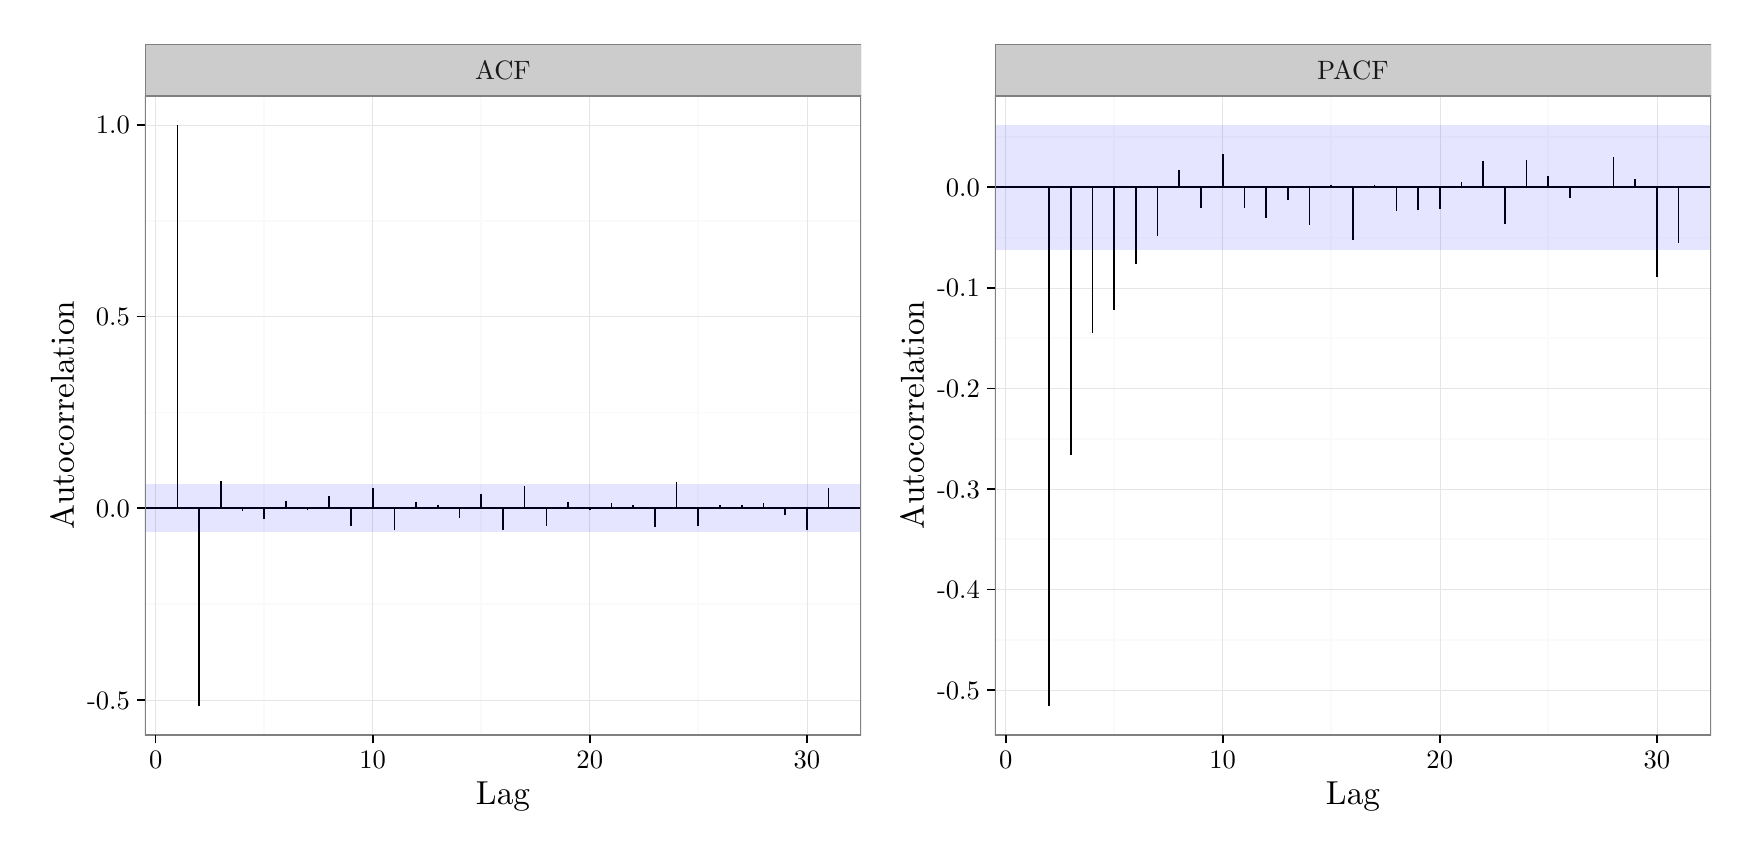
\begin{tikzpicture}[x=1pt,y=1pt]
\definecolor{fillColor}{RGB}{255,255,255}
\path[use as bounding box,fill=fillColor,fill opacity=0.00] (0,0) rectangle (614.29,289.08);
\begin{scope}
\path[clip] (  0.00,  0.00) rectangle (307.15,289.08);
\definecolor{drawColor}{RGB}{255,255,255}
\definecolor{fillColor}{RGB}{255,255,255}

\path[draw=drawColor,line width= 0.6pt,line join=round,line cap=round,fill=fillColor] (  0.00,  0.00) rectangle (307.15,289.08);
\end{scope}
\begin{scope}
\path[clip] ( 42.33, 33.48) rectangle (301.15,264.47);
\definecolor{fillColor}{RGB}{255,255,255}

\path[fill=fillColor] ( 42.33, 33.48) rectangle (301.15,264.47);
\definecolor{drawColor}{gray}{0.98}

\path[draw=drawColor,line width= 0.6pt,line join=round] ( 42.33, 80.78) --
	(301.15, 80.78);

\path[draw=drawColor,line width= 0.6pt,line join=round] ( 42.33,150.06) --
	(301.15,150.06);

\path[draw=drawColor,line width= 0.6pt,line join=round] ( 42.33,219.33) --
	(301.15,219.33);

\path[draw=drawColor,line width= 0.6pt,line join=round] ( 85.46, 33.48) --
	( 85.46,264.47);

\path[draw=drawColor,line width= 0.6pt,line join=round] (163.89, 33.48) --
	(163.89,264.47);

\path[draw=drawColor,line width= 0.6pt,line join=round] (242.32, 33.48) --
	(242.32,264.47);
\definecolor{drawColor}{gray}{0.90}

\path[draw=drawColor,line width= 0.2pt,line join=round] ( 42.33, 46.15) --
	(301.15, 46.15);

\path[draw=drawColor,line width= 0.2pt,line join=round] ( 42.33,115.42) --
	(301.15,115.42);

\path[draw=drawColor,line width= 0.2pt,line join=round] ( 42.33,184.69) --
	(301.15,184.69);

\path[draw=drawColor,line width= 0.2pt,line join=round] ( 42.33,253.97) --
	(301.15,253.97);

\path[draw=drawColor,line width= 0.2pt,line join=round] ( 46.25, 33.48) --
	( 46.25,264.47);

\path[draw=drawColor,line width= 0.2pt,line join=round] (124.68, 33.48) --
	(124.68,264.47);

\path[draw=drawColor,line width= 0.2pt,line join=round] (203.11, 33.48) --
	(203.11,264.47);

\path[draw=drawColor,line width= 0.2pt,line join=round] (281.54, 33.48) --
	(281.54,264.47);
\definecolor{drawColor}{RGB}{0,0,0}

\path[draw=drawColor,line width= 0.6pt,line join=round] ( 42.33,115.42) -- (301.15,115.42);

\path[draw=drawColor,line width= 0.6pt,line join=round] ( 54.09,253.97) -- ( 54.09,115.42);

\path[draw=drawColor,line width= 0.6pt,line join=round] ( 61.94, 43.98) -- ( 61.94,115.42);

\path[draw=drawColor,line width= 0.6pt,line join=round] ( 69.78,125.15) -- ( 69.78,115.42);

\path[draw=drawColor,line width= 0.6pt,line join=round] ( 77.62,114.42) -- ( 77.62,115.42);

\path[draw=drawColor,line width= 0.6pt,line join=round] ( 85.46,111.67) -- ( 85.46,115.42);

\path[draw=drawColor,line width= 0.6pt,line join=round] ( 93.31,118.06) -- ( 93.31,115.42);

\path[draw=drawColor,line width= 0.6pt,line join=round] (101.15,114.71) -- (101.15,115.42);

\path[draw=drawColor,line width= 0.6pt,line join=round] (108.99,119.95) -- (108.99,115.42);

\path[draw=drawColor,line width= 0.6pt,line join=round] (116.84,109.14) -- (116.84,115.42);

\path[draw=drawColor,line width= 0.6pt,line join=round] (124.68,122.62) -- (124.68,115.42);

\path[draw=drawColor,line width= 0.6pt,line join=round] (132.52,107.49) -- (132.52,115.42);

\path[draw=drawColor,line width= 0.6pt,line join=round] (140.37,117.71) -- (140.37,115.42);

\path[draw=drawColor,line width= 0.6pt,line join=round] (148.21,116.65) -- (148.21,115.42);

\path[draw=drawColor,line width= 0.6pt,line join=round] (156.05,111.94) -- (156.05,115.42);

\path[draw=drawColor,line width= 0.6pt,line join=round] (163.89,120.61) -- (163.89,115.42);

\path[draw=drawColor,line width= 0.6pt,line join=round] (171.74,107.67) -- (171.74,115.42);

\path[draw=drawColor,line width= 0.6pt,line join=round] (179.58,123.40) -- (179.58,115.42);

\path[draw=drawColor,line width= 0.6pt,line join=round] (187.42,109.10) -- (187.42,115.42);

\path[draw=drawColor,line width= 0.6pt,line join=round] (195.27,117.71) -- (195.27,115.42);

\path[draw=drawColor,line width= 0.6pt,line join=round] (203.11,114.68) -- (203.11,115.42);

\path[draw=drawColor,line width= 0.6pt,line join=round] (210.95,117.40) -- (210.95,115.42);

\path[draw=drawColor,line width= 0.6pt,line join=round] (218.80,116.58) -- (218.80,115.42);

\path[draw=drawColor,line width= 0.6pt,line join=round] (226.64,108.61) -- (226.64,115.42);

\path[draw=drawColor,line width= 0.6pt,line join=round] (234.48,125.05) -- (234.48,115.42);

\path[draw=drawColor,line width= 0.6pt,line join=round] (242.32,109.06) -- (242.32,115.42);

\path[draw=drawColor,line width= 0.6pt,line join=round] (250.17,116.58) -- (250.17,115.42);

\path[draw=drawColor,line width= 0.6pt,line join=round] (258.01,116.56) -- (258.01,115.42);

\path[draw=drawColor,line width= 0.6pt,line join=round] (265.85,117.17) -- (265.85,115.42);

\path[draw=drawColor,line width= 0.6pt,line join=round] (273.70,113.02) -- (273.70,115.42);

\path[draw=drawColor,line width= 0.6pt,line join=round] (281.54,107.69) -- (281.54,115.42);

\path[draw=drawColor,line width= 0.6pt,line join=round] (289.38,122.84) -- (289.38,115.42);
\definecolor{fillColor}{RGB}{0,0,255}

\path[fill=fillColor,fill opacity=0.10] ( 42.33,106.83) rectangle (301.15,124.01);
\definecolor{drawColor}{gray}{0.50}

\path[draw=drawColor,line width= 0.6pt,line join=round,line cap=round] ( 42.33, 33.48) rectangle (301.15,264.47);
\end{scope}
\begin{scope}
\path[clip] ( 42.33,264.47) rectangle (301.15,283.08);
\definecolor{drawColor}{gray}{0.50}
\definecolor{fillColor}{gray}{0.80}

\path[draw=drawColor,line width= 0.2pt,line join=round,line cap=round,fill=fillColor] ( 42.33,264.47) rectangle (301.15,283.08);
\definecolor{drawColor}{gray}{0.10}

\node[text=drawColor,anchor=base,inner sep=0pt, outer sep=0pt, scale=  0.96] at (171.74,270.47) {ACF};
\end{scope}
\begin{scope}
\path[clip] (  0.00,  0.00) rectangle (614.29,289.08);
\definecolor{drawColor}{RGB}{0,0,0}

\node[text=drawColor,anchor=base east,inner sep=0pt, outer sep=0pt, scale=  0.96] at ( 36.93, 42.84) {-0.5};

\node[text=drawColor,anchor=base east,inner sep=0pt, outer sep=0pt, scale=  0.96] at ( 36.93,112.11) {0.0};

\node[text=drawColor,anchor=base east,inner sep=0pt, outer sep=0pt, scale=  0.96] at ( 36.93,181.39) {0.5};

\node[text=drawColor,anchor=base east,inner sep=0pt, outer sep=0pt, scale=  0.96] at ( 36.93,250.66) {1.0};
\end{scope}
\begin{scope}
\path[clip] (  0.00,  0.00) rectangle (614.29,289.08);
\definecolor{drawColor}{RGB}{0,0,0}

\path[draw=drawColor,line width= 0.6pt,line join=round] ( 39.33, 46.15) --
	( 42.33, 46.15);

\path[draw=drawColor,line width= 0.6pt,line join=round] ( 39.33,115.42) --
	( 42.33,115.42);

\path[draw=drawColor,line width= 0.6pt,line join=round] ( 39.33,184.69) --
	( 42.33,184.69);

\path[draw=drawColor,line width= 0.6pt,line join=round] ( 39.33,253.97) --
	( 42.33,253.97);
\end{scope}
\begin{scope}
\path[clip] (  0.00,  0.00) rectangle (614.29,289.08);
\definecolor{drawColor}{RGB}{0,0,0}

\path[draw=drawColor,line width= 0.6pt,line join=round] ( 46.25, 30.48) --
	( 46.25, 33.48);

\path[draw=drawColor,line width= 0.6pt,line join=round] (124.68, 30.48) --
	(124.68, 33.48);

\path[draw=drawColor,line width= 0.6pt,line join=round] (203.11, 30.48) --
	(203.11, 33.48);

\path[draw=drawColor,line width= 0.6pt,line join=round] (281.54, 30.48) --
	(281.54, 33.48);
\end{scope}
\begin{scope}
\path[clip] (  0.00,  0.00) rectangle (614.29,289.08);
\definecolor{drawColor}{RGB}{0,0,0}

\node[text=drawColor,anchor=base,inner sep=0pt, outer sep=0pt, scale=  0.96] at ( 46.25, 21.46) {0};

\node[text=drawColor,anchor=base,inner sep=0pt, outer sep=0pt, scale=  0.96] at (124.68, 21.46) {10};

\node[text=drawColor,anchor=base,inner sep=0pt, outer sep=0pt, scale=  0.96] at (203.11, 21.46) {20};

\node[text=drawColor,anchor=base,inner sep=0pt, outer sep=0pt, scale=  0.96] at (281.54, 21.46) {30};
\end{scope}
\begin{scope}
\path[clip] (  0.00,  0.00) rectangle (614.29,289.08);
\definecolor{drawColor}{RGB}{0,0,0}

\node[text=drawColor,anchor=base,inner sep=0pt, outer sep=0pt, scale=  1.20] at (171.74,  8.40) {Lag};
\end{scope}
\begin{scope}
\path[clip] (  0.00,  0.00) rectangle (614.29,289.08);
\definecolor{drawColor}{RGB}{0,0,0}

\node[text=drawColor,rotate= 90.00,anchor=base,inner sep=0pt, outer sep=0pt, scale=  1.20] at ( 16.66,148.97) {Autocorrelation};
\end{scope}
\begin{scope}
\path[clip] (307.15,  0.00) rectangle (614.29,289.08);
\definecolor{drawColor}{RGB}{255,255,255}
\definecolor{fillColor}{RGB}{255,255,255}

\path[draw=drawColor,line width= 0.6pt,line join=round,line cap=round,fill=fillColor] (307.15,  0.00) rectangle (614.29,289.08);
\end{scope}
\begin{scope}
\path[clip] (349.48, 33.48) rectangle (608.30,264.47);
\definecolor{fillColor}{RGB}{255,255,255}

\path[fill=fillColor] (349.48, 33.48) rectangle (608.29,264.47);
\definecolor{drawColor}{gray}{0.98}

\path[draw=drawColor,line width= 0.6pt,line join=round] (349.48, 67.85) --
	(608.30, 67.85);

\path[draw=drawColor,line width= 0.6pt,line join=round] (349.48,104.20) --
	(608.30,104.20);

\path[draw=drawColor,line width= 0.6pt,line join=round] (349.48,140.55) --
	(608.30,140.55);

\path[draw=drawColor,line width= 0.6pt,line join=round] (349.48,176.91) --
	(608.30,176.91);

\path[draw=drawColor,line width= 0.6pt,line join=round] (349.48,213.26) --
	(608.30,213.26);

\path[draw=drawColor,line width= 0.6pt,line join=round] (349.48,249.61) --
	(608.30,249.61);

\path[draw=drawColor,line width= 0.6pt,line join=round] (392.61, 33.48) --
	(392.61,264.47);

\path[draw=drawColor,line width= 0.6pt,line join=round] (471.04, 33.48) --
	(471.04,264.47);

\path[draw=drawColor,line width= 0.6pt,line join=round] (549.47, 33.48) --
	(549.47,264.47);
\definecolor{drawColor}{gray}{0.90}

\path[draw=drawColor,line width= 0.2pt,line join=round] (349.48, 49.67) --
	(608.30, 49.67);

\path[draw=drawColor,line width= 0.2pt,line join=round] (349.48, 86.03) --
	(608.30, 86.03);

\path[draw=drawColor,line width= 0.2pt,line join=round] (349.48,122.38) --
	(608.30,122.38);

\path[draw=drawColor,line width= 0.2pt,line join=round] (349.48,158.73) --
	(608.30,158.73);

\path[draw=drawColor,line width= 0.2pt,line join=round] (349.48,195.08) --
	(608.30,195.08);

\path[draw=drawColor,line width= 0.2pt,line join=round] (349.48,231.44) --
	(608.30,231.44);

\path[draw=drawColor,line width= 0.2pt,line join=round] (353.40, 33.48) --
	(353.40,264.47);

\path[draw=drawColor,line width= 0.2pt,line join=round] (431.83, 33.48) --
	(431.83,264.47);

\path[draw=drawColor,line width= 0.2pt,line join=round] (510.26, 33.48) --
	(510.26,264.47);

\path[draw=drawColor,line width= 0.2pt,line join=round] (588.69, 33.48) --
	(588.69,264.47);
\definecolor{drawColor}{RGB}{0,0,0}

\path[draw=drawColor,line width= 0.6pt,line join=round] (349.48,231.44) -- (608.30,231.44);

\path[draw=drawColor,line width= 0.6pt,line join=round] (369.08, 43.98) -- (369.08,231.44);

\path[draw=drawColor,line width= 0.6pt,line join=round] (376.93,134.52) -- (376.93,231.44);

\path[draw=drawColor,line width= 0.6pt,line join=round] (384.77,178.73) -- (384.77,231.44);

\path[draw=drawColor,line width= 0.6pt,line join=round] (392.61,187.04) -- (392.61,231.44);

\path[draw=drawColor,line width= 0.6pt,line join=round] (400.45,203.81) -- (400.45,231.44);

\path[draw=drawColor,line width= 0.6pt,line join=round] (408.30,213.84) -- (408.30,231.44);

\path[draw=drawColor,line width= 0.6pt,line join=round] (416.14,237.66) -- (416.14,231.44);

\path[draw=drawColor,line width= 0.6pt,line join=round] (423.98,223.96) -- (423.98,231.44);

\path[draw=drawColor,line width= 0.6pt,line join=round] (431.83,243.49) -- (431.83,231.44);

\path[draw=drawColor,line width= 0.6pt,line join=round] (439.67,223.91) -- (439.67,231.44);

\path[draw=drawColor,line width= 0.6pt,line join=round] (447.51,220.41) -- (447.51,231.44);

\path[draw=drawColor,line width= 0.6pt,line join=round] (455.36,226.74) -- (455.36,231.44);

\path[draw=drawColor,line width= 0.6pt,line join=round] (463.20,217.87) -- (463.20,231.44);

\path[draw=drawColor,line width= 0.6pt,line join=round] (471.04,232.39) -- (471.04,231.44);

\path[draw=drawColor,line width= 0.6pt,line join=round] (478.89,212.33) -- (478.89,231.44);

\path[draw=drawColor,line width= 0.6pt,line join=round] (486.73,232.18) -- (486.73,231.44);

\path[draw=drawColor,line width= 0.6pt,line join=round] (494.57,222.99) -- (494.57,231.44);

\path[draw=drawColor,line width= 0.6pt,line join=round] (502.41,223.13) -- (502.41,231.44);

\path[draw=drawColor,line width= 0.6pt,line join=round] (510.26,223.65) -- (510.26,231.44);

\path[draw=drawColor,line width= 0.6pt,line join=round] (518.10,233.25) -- (518.10,231.44);

\path[draw=drawColor,line width= 0.6pt,line join=round] (525.94,240.72) -- (525.94,231.44);

\path[draw=drawColor,line width= 0.6pt,line join=round] (533.79,218.07) -- (533.79,231.44);

\path[draw=drawColor,line width= 0.6pt,line join=round] (541.63,241.16) -- (541.63,231.44);

\path[draw=drawColor,line width= 0.6pt,line join=round] (549.47,235.64) -- (549.47,231.44);

\path[draw=drawColor,line width= 0.6pt,line join=round] (557.32,227.70) -- (557.32,231.44);

\path[draw=drawColor,line width= 0.6pt,line join=round] (565.16,232.00) -- (565.16,231.44);

\path[draw=drawColor,line width= 0.6pt,line join=round] (573.00,242.17) -- (573.00,231.44);

\path[draw=drawColor,line width= 0.6pt,line join=round] (580.84,234.35) -- (580.84,231.44);

\path[draw=drawColor,line width= 0.6pt,line join=round] (588.69,199.11) -- (588.69,231.44);

\path[draw=drawColor,line width= 0.6pt,line join=round] (596.53,211.23) -- (596.53,231.44);
\definecolor{fillColor}{RGB}{0,0,255}

\path[fill=fillColor,fill opacity=0.10] (349.48,208.91) rectangle (608.29,253.97);
\definecolor{drawColor}{gray}{0.50}

\path[draw=drawColor,line width= 0.6pt,line join=round,line cap=round] (349.48, 33.48) rectangle (608.29,264.47);
\end{scope}
\begin{scope}
\path[clip] (349.48,264.47) rectangle (608.30,283.08);
\definecolor{drawColor}{gray}{0.50}
\definecolor{fillColor}{gray}{0.80}

\path[draw=drawColor,line width= 0.2pt,line join=round,line cap=round,fill=fillColor] (349.48,264.47) rectangle (608.29,283.08);
\definecolor{drawColor}{gray}{0.10}

\node[text=drawColor,anchor=base,inner sep=0pt, outer sep=0pt, scale=  0.96] at (478.89,270.47) {PACF};
\end{scope}
\begin{scope}
\path[clip] (  0.00,  0.00) rectangle (614.29,289.08);
\definecolor{drawColor}{RGB}{0,0,0}

\node[text=drawColor,anchor=base east,inner sep=0pt, outer sep=0pt, scale=  0.96] at (344.08, 46.37) {-0.5};

\node[text=drawColor,anchor=base east,inner sep=0pt, outer sep=0pt, scale=  0.96] at (344.08, 82.72) {-0.4};

\node[text=drawColor,anchor=base east,inner sep=0pt, outer sep=0pt, scale=  0.96] at (344.08,119.07) {-0.3};

\node[text=drawColor,anchor=base east,inner sep=0pt, outer sep=0pt, scale=  0.96] at (344.08,155.43) {-0.2};

\node[text=drawColor,anchor=base east,inner sep=0pt, outer sep=0pt, scale=  0.96] at (344.08,191.78) {-0.1};

\node[text=drawColor,anchor=base east,inner sep=0pt, outer sep=0pt, scale=  0.96] at (344.08,228.13) {0.0};
\end{scope}
\begin{scope}
\path[clip] (  0.00,  0.00) rectangle (614.29,289.08);
\definecolor{drawColor}{RGB}{0,0,0}

\path[draw=drawColor,line width= 0.6pt,line join=round] (346.48, 49.67) --
	(349.48, 49.67);

\path[draw=drawColor,line width= 0.6pt,line join=round] (346.48, 86.03) --
	(349.48, 86.03);

\path[draw=drawColor,line width= 0.6pt,line join=round] (346.48,122.38) --
	(349.48,122.38);

\path[draw=drawColor,line width= 0.6pt,line join=round] (346.48,158.73) --
	(349.48,158.73);

\path[draw=drawColor,line width= 0.6pt,line join=round] (346.48,195.08) --
	(349.48,195.08);

\path[draw=drawColor,line width= 0.6pt,line join=round] (346.48,231.44) --
	(349.48,231.44);
\end{scope}
\begin{scope}
\path[clip] (  0.00,  0.00) rectangle (614.29,289.08);
\definecolor{drawColor}{RGB}{0,0,0}

\path[draw=drawColor,line width= 0.6pt,line join=round] (353.40, 30.48) --
	(353.40, 33.48);

\path[draw=drawColor,line width= 0.6pt,line join=round] (431.83, 30.48) --
	(431.83, 33.48);

\path[draw=drawColor,line width= 0.6pt,line join=round] (510.26, 30.48) --
	(510.26, 33.48);

\path[draw=drawColor,line width= 0.6pt,line join=round] (588.69, 30.48) --
	(588.69, 33.48);
\end{scope}
\begin{scope}
\path[clip] (  0.00,  0.00) rectangle (614.29,289.08);
\definecolor{drawColor}{RGB}{0,0,0}

\node[text=drawColor,anchor=base,inner sep=0pt, outer sep=0pt, scale=  0.96] at (353.40, 21.46) {0};

\node[text=drawColor,anchor=base,inner sep=0pt, outer sep=0pt, scale=  0.96] at (431.83, 21.46) {10};

\node[text=drawColor,anchor=base,inner sep=0pt, outer sep=0pt, scale=  0.96] at (510.26, 21.46) {20};

\node[text=drawColor,anchor=base,inner sep=0pt, outer sep=0pt, scale=  0.96] at (588.69, 21.46) {30};
\end{scope}
\begin{scope}
\path[clip] (  0.00,  0.00) rectangle (614.29,289.08);
\definecolor{drawColor}{RGB}{0,0,0}

\node[text=drawColor,anchor=base,inner sep=0pt, outer sep=0pt, scale=  1.20] at (478.89,  8.40) {Lag};
\end{scope}
\begin{scope}
\path[clip] (  0.00,  0.00) rectangle (614.29,289.08);
\definecolor{drawColor}{RGB}{0,0,0}

\node[text=drawColor,rotate= 90.00,anchor=base,inner sep=0pt, outer sep=0pt, scale=  1.20] at (323.81,148.97) {Autocorrelation};
\end{scope}
\end{tikzpicture}
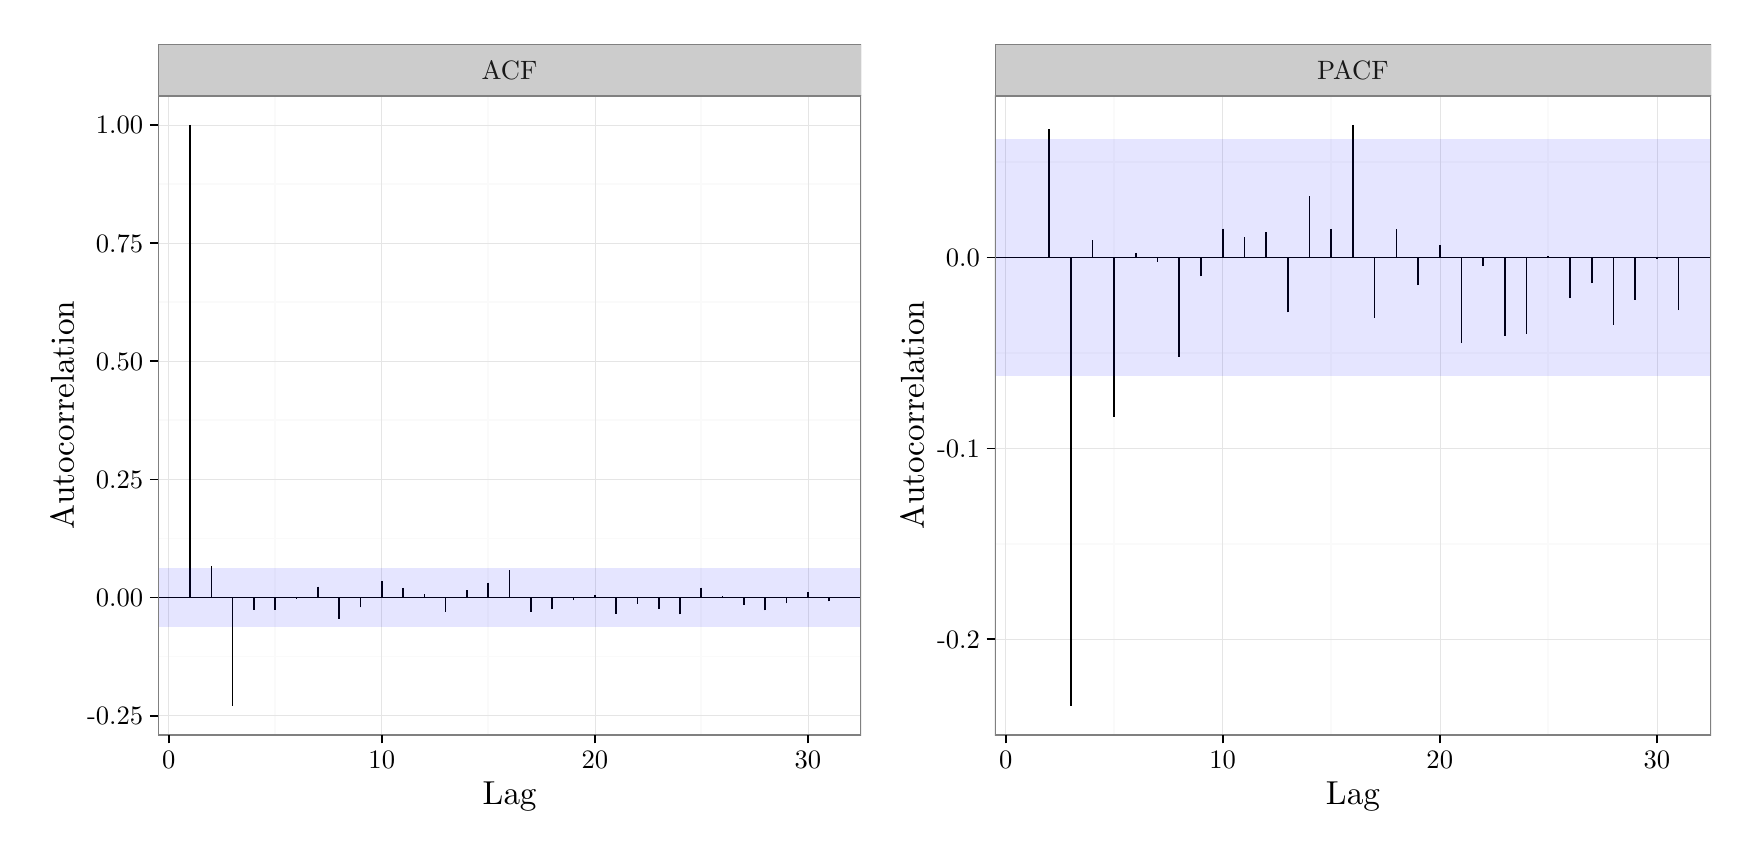
\begin{tikzpicture}[x=1pt,y=1pt]
\definecolor{fillColor}{RGB}{255,255,255}
\path[use as bounding box,fill=fillColor,fill opacity=0.00] (0,0) rectangle (614.29,289.08);
\begin{scope}
\path[clip] (  0.00,  0.00) rectangle (307.15,289.08);
\definecolor{drawColor}{RGB}{255,255,255}
\definecolor{fillColor}{RGB}{255,255,255}

\path[draw=drawColor,line width= 0.6pt,line join=round,line cap=round,fill=fillColor] (  0.00,  0.00) rectangle (307.15,289.08);
\end{scope}
\begin{scope}
\path[clip] ( 47.13, 33.48) rectangle (301.15,264.47);
\definecolor{fillColor}{RGB}{255,255,255}

\path[fill=fillColor] ( 47.13, 33.48) rectangle (301.15,264.47);
\definecolor{drawColor}{gray}{0.98}

\path[draw=drawColor,line width= 0.6pt,line join=round] ( 47.13, 61.80) --
	(301.15, 61.80);

\path[draw=drawColor,line width= 0.6pt,line join=round] ( 47.13,104.50) --
	(301.15,104.50);

\path[draw=drawColor,line width= 0.6pt,line join=round] ( 47.13,147.21) --
	(301.15,147.21);

\path[draw=drawColor,line width= 0.6pt,line join=round] ( 47.13,189.91) --
	(301.15,189.91);

\path[draw=drawColor,line width= 0.6pt,line join=round] ( 47.13,232.62) --
	(301.15,232.62);

\path[draw=drawColor,line width= 0.6pt,line join=round] ( 89.46, 33.48) --
	( 89.46,264.47);

\path[draw=drawColor,line width= 0.6pt,line join=round] (166.44, 33.48) --
	(166.44,264.47);

\path[draw=drawColor,line width= 0.6pt,line join=round] (243.42, 33.48) --
	(243.42,264.47);
\definecolor{drawColor}{gray}{0.90}

\path[draw=drawColor,line width= 0.2pt,line join=round] ( 47.13, 40.45) --
	(301.15, 40.45);

\path[draw=drawColor,line width= 0.2pt,line join=round] ( 47.13, 83.15) --
	(301.15, 83.15);

\path[draw=drawColor,line width= 0.2pt,line join=round] ( 47.13,125.85) --
	(301.15,125.85);

\path[draw=drawColor,line width= 0.2pt,line join=round] ( 47.13,168.56) --
	(301.15,168.56);

\path[draw=drawColor,line width= 0.2pt,line join=round] ( 47.13,211.26) --
	(301.15,211.26);

\path[draw=drawColor,line width= 0.2pt,line join=round] ( 47.13,253.97) --
	(301.15,253.97);

\path[draw=drawColor,line width= 0.2pt,line join=round] ( 50.98, 33.48) --
	( 50.98,264.47);

\path[draw=drawColor,line width= 0.2pt,line join=round] (127.95, 33.48) --
	(127.95,264.47);

\path[draw=drawColor,line width= 0.2pt,line join=round] (204.93, 33.48) --
	(204.93,264.47);

\path[draw=drawColor,line width= 0.2pt,line join=round] (281.90, 33.48) --
	(281.90,264.47);
\definecolor{drawColor}{RGB}{0,0,0}

\path[draw=drawColor,line width= 0.6pt,line join=round] ( 47.13, 83.15) -- (301.15, 83.15);

\path[draw=drawColor,line width= 0.6pt,line join=round] ( 58.67,253.97) -- ( 58.67, 83.15);

\path[draw=drawColor,line width= 0.6pt,line join=round] ( 66.37, 94.64) -- ( 66.37, 83.15);

\path[draw=drawColor,line width= 0.6pt,line join=round] ( 74.07, 43.98) -- ( 74.07, 83.15);

\path[draw=drawColor,line width= 0.6pt,line join=round] ( 81.77, 78.66) -- ( 81.77, 83.15);

\path[draw=drawColor,line width= 0.6pt,line join=round] ( 89.46, 78.69) -- ( 89.46, 83.15);

\path[draw=drawColor,line width= 0.6pt,line join=round] ( 97.16, 82.70) -- ( 97.16, 83.15);

\path[draw=drawColor,line width= 0.6pt,line join=round] (104.86, 87.13) -- (104.86, 83.15);

\path[draw=drawColor,line width= 0.6pt,line join=round] (112.56, 75.50) -- (112.56, 83.15);

\path[draw=drawColor,line width= 0.6pt,line join=round] (120.25, 79.63) -- (120.25, 83.15);

\path[draw=drawColor,line width= 0.6pt,line join=round] (127.95, 89.22) -- (127.95, 83.15);

\path[draw=drawColor,line width= 0.6pt,line join=round] (135.65, 86.66) -- (135.65, 83.15);

\path[draw=drawColor,line width= 0.6pt,line join=round] (143.35, 84.40) -- (143.35, 83.15);

\path[draw=drawColor,line width= 0.6pt,line join=round] (151.04, 78.00) -- (151.04, 83.15);

\path[draw=drawColor,line width= 0.6pt,line join=round] (158.74, 85.82) -- (158.74, 83.15);

\path[draw=drawColor,line width= 0.6pt,line join=round] (166.44, 88.51) -- (166.44, 83.15);

\path[draw=drawColor,line width= 0.6pt,line join=round] (174.14, 93.07) -- (174.14, 83.15);

\path[draw=drawColor,line width= 0.6pt,line join=round] (181.83, 78.08) -- (181.83, 83.15);

\path[draw=drawColor,line width= 0.6pt,line join=round] (189.53, 78.84) -- (189.53, 83.15);

\path[draw=drawColor,line width= 0.6pt,line join=round] (197.23, 82.22) -- (197.23, 83.15);

\path[draw=drawColor,line width= 0.6pt,line join=round] (204.93, 83.90) -- (204.93, 83.15);

\path[draw=drawColor,line width= 0.6pt,line join=round] (212.63, 77.25) -- (212.63, 83.15);

\path[draw=drawColor,line width= 0.6pt,line join=round] (220.32, 80.94) -- (220.32, 83.15);

\path[draw=drawColor,line width= 0.6pt,line join=round] (228.02, 78.93) -- (228.02, 83.15);

\path[draw=drawColor,line width= 0.6pt,line join=round] (235.72, 77.03) -- (235.72, 83.15);

\path[draw=drawColor,line width= 0.6pt,line join=round] (243.42, 86.70) -- (243.42, 83.15);

\path[draw=drawColor,line width= 0.6pt,line join=round] (251.11, 83.71) -- (251.11, 83.15);

\path[draw=drawColor,line width= 0.6pt,line join=round] (258.81, 80.52) -- (258.81, 83.15);

\path[draw=drawColor,line width= 0.6pt,line join=round] (266.51, 78.53) -- (266.51, 83.15);

\path[draw=drawColor,line width= 0.6pt,line join=round] (274.21, 81.01) -- (274.21, 83.15);

\path[draw=drawColor,line width= 0.6pt,line join=round] (281.90, 85.15) -- (281.90, 83.15);

\path[draw=drawColor,line width= 0.6pt,line join=round] (289.60, 81.81) -- (289.60, 83.15);
\definecolor{fillColor}{RGB}{0,0,255}

\path[fill=fillColor,fill opacity=0.10] ( 47.13, 72.56) rectangle (301.15, 93.74);
\definecolor{drawColor}{gray}{0.50}

\path[draw=drawColor,line width= 0.6pt,line join=round,line cap=round] ( 47.13, 33.48) rectangle (301.15,264.47);
\end{scope}
\begin{scope}
\path[clip] ( 47.13,264.47) rectangle (301.15,283.08);
\definecolor{drawColor}{gray}{0.50}
\definecolor{fillColor}{gray}{0.80}

\path[draw=drawColor,line width= 0.2pt,line join=round,line cap=round,fill=fillColor] ( 47.13,264.47) rectangle (301.15,283.08);
\definecolor{drawColor}{gray}{0.10}

\node[text=drawColor,anchor=base,inner sep=0pt, outer sep=0pt, scale=  0.96] at (174.14,270.47) {ACF};
\end{scope}
\begin{scope}
\path[clip] (  0.00,  0.00) rectangle (614.29,289.08);
\definecolor{drawColor}{RGB}{0,0,0}

\node[text=drawColor,anchor=base east,inner sep=0pt, outer sep=0pt, scale=  0.96] at ( 41.73, 37.14) {-0.25};

\node[text=drawColor,anchor=base east,inner sep=0pt, outer sep=0pt, scale=  0.96] at ( 41.73, 79.84) {0.00};

\node[text=drawColor,anchor=base east,inner sep=0pt, outer sep=0pt, scale=  0.96] at ( 41.73,122.55) {0.25};

\node[text=drawColor,anchor=base east,inner sep=0pt, outer sep=0pt, scale=  0.96] at ( 41.73,165.25) {0.50};

\node[text=drawColor,anchor=base east,inner sep=0pt, outer sep=0pt, scale=  0.96] at ( 41.73,207.96) {0.75};

\node[text=drawColor,anchor=base east,inner sep=0pt, outer sep=0pt, scale=  0.96] at ( 41.73,250.66) {1.00};
\end{scope}
\begin{scope}
\path[clip] (  0.00,  0.00) rectangle (614.29,289.08);
\definecolor{drawColor}{RGB}{0,0,0}

\path[draw=drawColor,line width= 0.6pt,line join=round] ( 44.13, 40.45) --
	( 47.13, 40.45);

\path[draw=drawColor,line width= 0.6pt,line join=round] ( 44.13, 83.15) --
	( 47.13, 83.15);

\path[draw=drawColor,line width= 0.6pt,line join=round] ( 44.13,125.85) --
	( 47.13,125.85);

\path[draw=drawColor,line width= 0.6pt,line join=round] ( 44.13,168.56) --
	( 47.13,168.56);

\path[draw=drawColor,line width= 0.6pt,line join=round] ( 44.13,211.26) --
	( 47.13,211.26);

\path[draw=drawColor,line width= 0.6pt,line join=round] ( 44.13,253.97) --
	( 47.13,253.97);
\end{scope}
\begin{scope}
\path[clip] (  0.00,  0.00) rectangle (614.29,289.08);
\definecolor{drawColor}{RGB}{0,0,0}

\path[draw=drawColor,line width= 0.6pt,line join=round] ( 50.98, 30.48) --
	( 50.98, 33.48);

\path[draw=drawColor,line width= 0.6pt,line join=round] (127.95, 30.48) --
	(127.95, 33.48);

\path[draw=drawColor,line width= 0.6pt,line join=round] (204.93, 30.48) --
	(204.93, 33.48);

\path[draw=drawColor,line width= 0.6pt,line join=round] (281.90, 30.48) --
	(281.90, 33.48);
\end{scope}
\begin{scope}
\path[clip] (  0.00,  0.00) rectangle (614.29,289.08);
\definecolor{drawColor}{RGB}{0,0,0}

\node[text=drawColor,anchor=base,inner sep=0pt, outer sep=0pt, scale=  0.96] at ( 50.98, 21.46) {0};

\node[text=drawColor,anchor=base,inner sep=0pt, outer sep=0pt, scale=  0.96] at (127.95, 21.46) {10};

\node[text=drawColor,anchor=base,inner sep=0pt, outer sep=0pt, scale=  0.96] at (204.93, 21.46) {20};

\node[text=drawColor,anchor=base,inner sep=0pt, outer sep=0pt, scale=  0.96] at (281.90, 21.46) {30};
\end{scope}
\begin{scope}
\path[clip] (  0.00,  0.00) rectangle (614.29,289.08);
\definecolor{drawColor}{RGB}{0,0,0}

\node[text=drawColor,anchor=base,inner sep=0pt, outer sep=0pt, scale=  1.20] at (174.14,  8.40) {Lag};
\end{scope}
\begin{scope}
\path[clip] (  0.00,  0.00) rectangle (614.29,289.08);
\definecolor{drawColor}{RGB}{0,0,0}

\node[text=drawColor,rotate= 90.00,anchor=base,inner sep=0pt, outer sep=0pt, scale=  1.20] at ( 16.66,148.97) {Autocorrelation};
\end{scope}
\begin{scope}
\path[clip] (307.15,  0.00) rectangle (614.29,289.08);
\definecolor{drawColor}{RGB}{255,255,255}
\definecolor{fillColor}{RGB}{255,255,255}

\path[draw=drawColor,line width= 0.6pt,line join=round,line cap=round,fill=fillColor] (307.15,  0.00) rectangle (614.29,289.08);
\end{scope}
\begin{scope}
\path[clip] (349.48, 33.48) rectangle (608.30,264.47);
\definecolor{fillColor}{RGB}{255,255,255}

\path[fill=fillColor] (349.48, 33.48) rectangle (608.29,264.47);
\definecolor{drawColor}{gray}{0.98}

\path[draw=drawColor,line width= 0.6pt,line join=round] (349.48, 33.57) --
	(608.30, 33.57);

\path[draw=drawColor,line width= 0.6pt,line join=round] (349.48,102.56) --
	(608.30,102.56);

\path[draw=drawColor,line width= 0.6pt,line join=round] (349.48,171.55) --
	(608.30,171.55);

\path[draw=drawColor,line width= 0.6pt,line join=round] (349.48,240.54) --
	(608.30,240.54);

\path[draw=drawColor,line width= 0.6pt,line join=round] (392.61, 33.48) --
	(392.61,264.47);

\path[draw=drawColor,line width= 0.6pt,line join=round] (471.04, 33.48) --
	(471.04,264.47);

\path[draw=drawColor,line width= 0.6pt,line join=round] (549.47, 33.48) --
	(549.47,264.47);
\definecolor{drawColor}{gray}{0.90}

\path[draw=drawColor,line width= 0.2pt,line join=round] (349.48, 68.07) --
	(608.30, 68.07);

\path[draw=drawColor,line width= 0.2pt,line join=round] (349.48,137.06) --
	(608.30,137.06);

\path[draw=drawColor,line width= 0.2pt,line join=round] (349.48,206.05) --
	(608.30,206.05);

\path[draw=drawColor,line width= 0.2pt,line join=round] (353.40, 33.48) --
	(353.40,264.47);

\path[draw=drawColor,line width= 0.2pt,line join=round] (431.83, 33.48) --
	(431.83,264.47);

\path[draw=drawColor,line width= 0.2pt,line join=round] (510.26, 33.48) --
	(510.26,264.47);

\path[draw=drawColor,line width= 0.2pt,line join=round] (588.69, 33.48) --
	(588.69,264.47);
\definecolor{drawColor}{RGB}{0,0,0}

\path[draw=drawColor,line width= 0.6pt,line join=round] (349.48,206.05) -- (608.30,206.05);

\path[draw=drawColor,line width= 0.6pt,line join=round] (369.08,252.44) -- (369.08,206.05);

\path[draw=drawColor,line width= 0.6pt,line join=round] (376.93, 43.98) -- (376.93,206.05);

\path[draw=drawColor,line width= 0.6pt,line join=round] (384.77,212.31) -- (384.77,206.05);

\path[draw=drawColor,line width= 0.6pt,line join=round] (392.61,148.46) -- (392.61,206.05);

\path[draw=drawColor,line width= 0.6pt,line join=round] (400.45,207.70) -- (400.45,206.05);

\path[draw=drawColor,line width= 0.6pt,line join=round] (408.30,204.52) -- (408.30,206.05);

\path[draw=drawColor,line width= 0.6pt,line join=round] (416.14,170.23) -- (416.14,206.05);

\path[draw=drawColor,line width= 0.6pt,line join=round] (423.98,199.20) -- (423.98,206.05);

\path[draw=drawColor,line width= 0.6pt,line join=round] (431.83,216.44) -- (431.83,206.05);

\path[draw=drawColor,line width= 0.6pt,line join=round] (439.67,213.37) -- (439.67,206.05);

\path[draw=drawColor,line width= 0.6pt,line join=round] (447.51,215.24) -- (447.51,206.05);

\path[draw=drawColor,line width= 0.6pt,line join=round] (455.36,186.20) -- (455.36,206.05);

\path[draw=drawColor,line width= 0.6pt,line join=round] (463.20,228.09) -- (463.20,206.05);

\path[draw=drawColor,line width= 0.6pt,line join=round] (471.04,216.34) -- (471.04,206.05);

\path[draw=drawColor,line width= 0.6pt,line join=round] (478.89,253.97) -- (478.89,206.05);

\path[draw=drawColor,line width= 0.6pt,line join=round] (486.73,184.33) -- (486.73,206.05);

\path[draw=drawColor,line width= 0.6pt,line join=round] (494.57,216.31) -- (494.57,206.05);

\path[draw=drawColor,line width= 0.6pt,line join=round] (502.41,196.04) -- (502.41,206.05);

\path[draw=drawColor,line width= 0.6pt,line join=round] (510.26,210.63) -- (510.26,206.05);

\path[draw=drawColor,line width= 0.6pt,line join=round] (518.10,175.13) -- (518.10,206.05);

\path[draw=drawColor,line width= 0.6pt,line join=round] (525.94,202.90) -- (525.94,206.05);

\path[draw=drawColor,line width= 0.6pt,line join=round] (533.79,177.69) -- (533.79,206.05);

\path[draw=drawColor,line width= 0.6pt,line join=round] (541.63,178.56) -- (541.63,206.05);

\path[draw=drawColor,line width= 0.6pt,line join=round] (549.47,206.47) -- (549.47,206.05);

\path[draw=drawColor,line width= 0.6pt,line join=round] (557.32,191.33) -- (557.32,206.05);

\path[draw=drawColor,line width= 0.6pt,line join=round] (565.16,196.79) -- (565.16,206.05);

\path[draw=drawColor,line width= 0.6pt,line join=round] (573.00,181.66) -- (573.00,206.05);

\path[draw=drawColor,line width= 0.6pt,line join=round] (580.84,190.75) -- (580.84,206.05);

\path[draw=drawColor,line width= 0.6pt,line join=round] (588.69,205.61) -- (588.69,206.05);

\path[draw=drawColor,line width= 0.6pt,line join=round] (596.53,187.02) -- (596.53,206.05);
\definecolor{fillColor}{RGB}{0,0,255}

\path[fill=fillColor,fill opacity=0.10] (349.48,163.29) rectangle (608.29,248.80);
\definecolor{drawColor}{gray}{0.50}

\path[draw=drawColor,line width= 0.6pt,line join=round,line cap=round] (349.48, 33.48) rectangle (608.29,264.47);
\end{scope}
\begin{scope}
\path[clip] (349.48,264.47) rectangle (608.30,283.08);
\definecolor{drawColor}{gray}{0.50}
\definecolor{fillColor}{gray}{0.80}

\path[draw=drawColor,line width= 0.2pt,line join=round,line cap=round,fill=fillColor] (349.48,264.47) rectangle (608.29,283.08);
\definecolor{drawColor}{gray}{0.10}

\node[text=drawColor,anchor=base,inner sep=0pt, outer sep=0pt, scale=  0.96] at (478.89,270.47) {PACF};
\end{scope}
\begin{scope}
\path[clip] (  0.00,  0.00) rectangle (614.29,289.08);
\definecolor{drawColor}{RGB}{0,0,0}

\node[text=drawColor,anchor=base east,inner sep=0pt, outer sep=0pt, scale=  0.96] at (344.08, 64.76) {-0.2};

\node[text=drawColor,anchor=base east,inner sep=0pt, outer sep=0pt, scale=  0.96] at (344.08,133.75) {-0.1};

\node[text=drawColor,anchor=base east,inner sep=0pt, outer sep=0pt, scale=  0.96] at (344.08,202.74) {0.0};
\end{scope}
\begin{scope}
\path[clip] (  0.00,  0.00) rectangle (614.29,289.08);
\definecolor{drawColor}{RGB}{0,0,0}

\path[draw=drawColor,line width= 0.6pt,line join=round] (346.48, 68.07) --
	(349.48, 68.07);

\path[draw=drawColor,line width= 0.6pt,line join=round] (346.48,137.06) --
	(349.48,137.06);

\path[draw=drawColor,line width= 0.6pt,line join=round] (346.48,206.05) --
	(349.48,206.05);
\end{scope}
\begin{scope}
\path[clip] (  0.00,  0.00) rectangle (614.29,289.08);
\definecolor{drawColor}{RGB}{0,0,0}

\path[draw=drawColor,line width= 0.6pt,line join=round] (353.40, 30.48) --
	(353.40, 33.48);

\path[draw=drawColor,line width= 0.6pt,line join=round] (431.83, 30.48) --
	(431.83, 33.48);

\path[draw=drawColor,line width= 0.6pt,line join=round] (510.26, 30.48) --
	(510.26, 33.48);

\path[draw=drawColor,line width= 0.6pt,line join=round] (588.69, 30.48) --
	(588.69, 33.48);
\end{scope}
\begin{scope}
\path[clip] (  0.00,  0.00) rectangle (614.29,289.08);
\definecolor{drawColor}{RGB}{0,0,0}

\node[text=drawColor,anchor=base,inner sep=0pt, outer sep=0pt, scale=  0.96] at (353.40, 21.46) {0};

\node[text=drawColor,anchor=base,inner sep=0pt, outer sep=0pt, scale=  0.96] at (431.83, 21.46) {10};

\node[text=drawColor,anchor=base,inner sep=0pt, outer sep=0pt, scale=  0.96] at (510.26, 21.46) {20};

\node[text=drawColor,anchor=base,inner sep=0pt, outer sep=0pt, scale=  0.96] at (588.69, 21.46) {30};
\end{scope}
\begin{scope}
\path[clip] (  0.00,  0.00) rectangle (614.29,289.08);
\definecolor{drawColor}{RGB}{0,0,0}

\node[text=drawColor,anchor=base,inner sep=0pt, outer sep=0pt, scale=  1.20] at (478.89,  8.40) {Lag};
\end{scope}
\begin{scope}
\path[clip] (  0.00,  0.00) rectangle (614.29,289.08);
\definecolor{drawColor}{RGB}{0,0,0}

\node[text=drawColor,rotate= 90.00,anchor=base,inner sep=0pt, outer sep=0pt, scale=  1.20] at (323.81,148.97) {Autocorrelation};
\end{scope}
\end{tikzpicture}
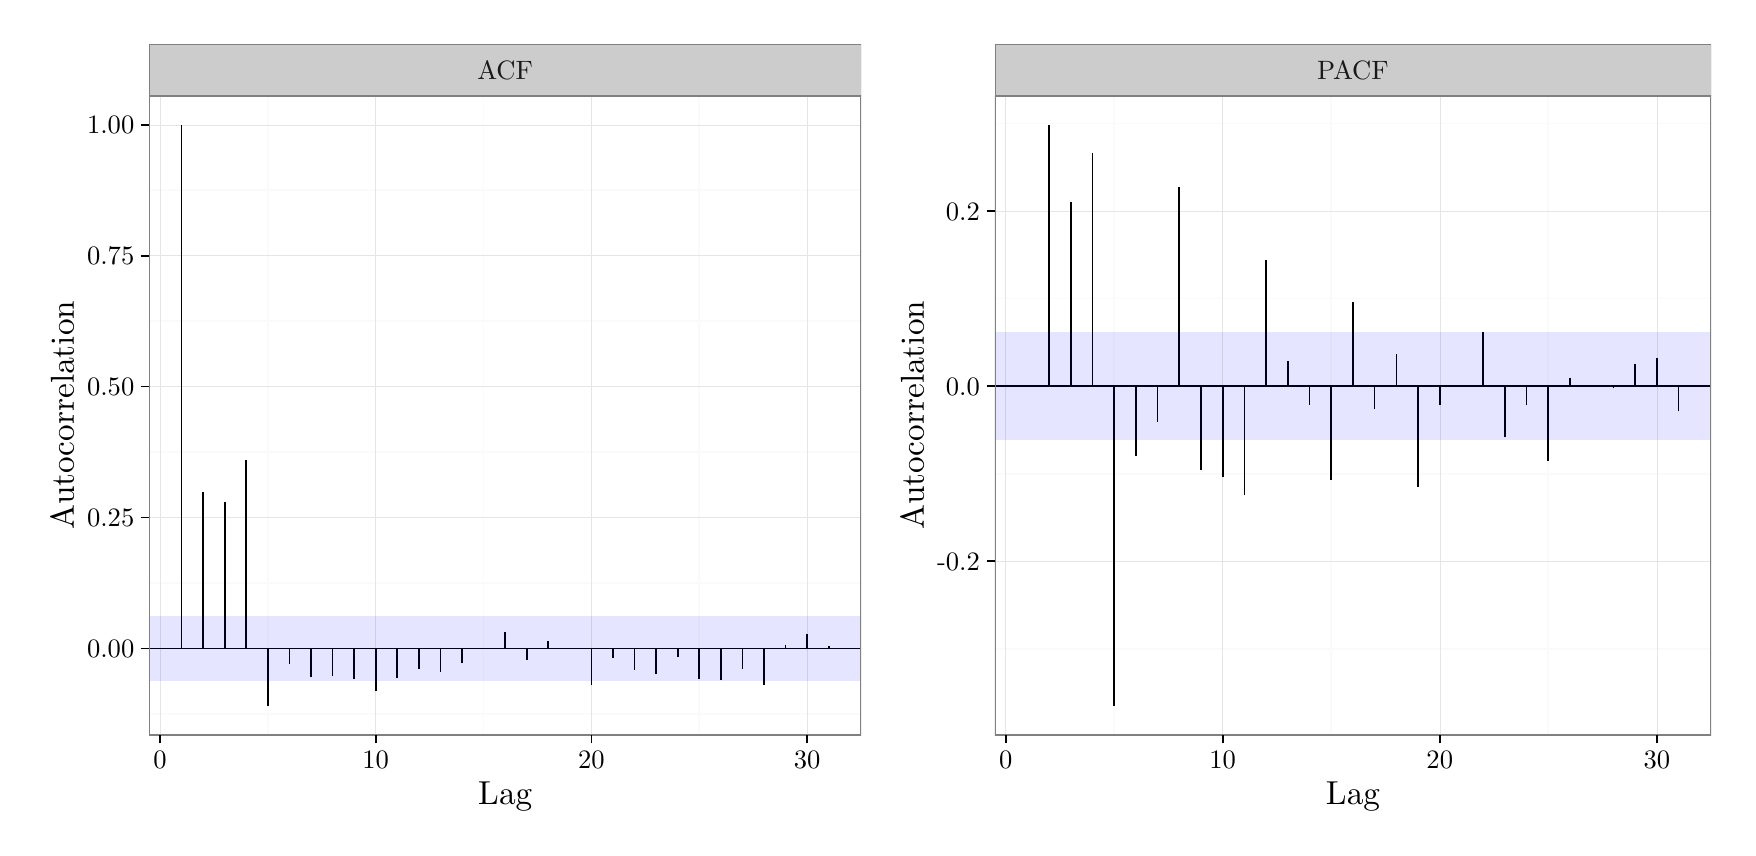
\begin{tikzpicture}[x=1pt,y=1pt]
\definecolor{fillColor}{RGB}{255,255,255}
\path[use as bounding box,fill=fillColor,fill opacity=0.00] (0,0) rectangle (614.29,289.08);
\begin{scope}
\path[clip] (  0.00,  0.00) rectangle (307.15,289.08);
\definecolor{drawColor}{RGB}{255,255,255}
\definecolor{fillColor}{RGB}{255,255,255}

\path[draw=drawColor,line width= 0.6pt,line join=round,line cap=round,fill=fillColor] ( -0.00,  0.00) rectangle (307.15,289.08);
\end{scope}
\begin{scope}
\path[clip] ( 43.93, 33.48) rectangle (301.15,264.47);
\definecolor{fillColor}{RGB}{255,255,255}

\path[fill=fillColor] ( 43.93, 33.48) rectangle (301.15,264.47);
\definecolor{drawColor}{gray}{0.98}

\path[draw=drawColor,line width= 0.6pt,line join=round] ( 43.93, 41.11) --
	(301.15, 41.11);

\path[draw=drawColor,line width= 0.6pt,line join=round] ( 43.93, 88.42) --
	(301.15, 88.42);

\path[draw=drawColor,line width= 0.6pt,line join=round] ( 43.93,135.72) --
	(301.15,135.72);

\path[draw=drawColor,line width= 0.6pt,line join=round] ( 43.93,183.02) --
	(301.15,183.02);

\path[draw=drawColor,line width= 0.6pt,line join=round] ( 43.93,230.32) --
	(301.15,230.32);

\path[draw=drawColor,line width= 0.6pt,line join=round] ( 86.80, 33.48) --
	( 86.80,264.47);

\path[draw=drawColor,line width= 0.6pt,line join=round] (164.74, 33.48) --
	(164.74,264.47);

\path[draw=drawColor,line width= 0.6pt,line join=round] (242.69, 33.48) --
	(242.69,264.47);
\definecolor{drawColor}{gray}{0.90}

\path[draw=drawColor,line width= 0.2pt,line join=round] ( 43.93, 64.76) --
	(301.15, 64.76);

\path[draw=drawColor,line width= 0.2pt,line join=round] ( 43.93,112.07) --
	(301.15,112.07);

\path[draw=drawColor,line width= 0.2pt,line join=round] ( 43.93,159.37) --
	(301.15,159.37);

\path[draw=drawColor,line width= 0.2pt,line join=round] ( 43.93,206.67) --
	(301.15,206.67);

\path[draw=drawColor,line width= 0.2pt,line join=round] ( 43.93,253.97) --
	(301.15,253.97);

\path[draw=drawColor,line width= 0.2pt,line join=round] ( 47.82, 33.48) --
	( 47.82,264.47);

\path[draw=drawColor,line width= 0.2pt,line join=round] (125.77, 33.48) --
	(125.77,264.47);

\path[draw=drawColor,line width= 0.2pt,line join=round] (203.72, 33.48) --
	(203.72,264.47);

\path[draw=drawColor,line width= 0.2pt,line join=round] (281.66, 33.48) --
	(281.66,264.47);
\definecolor{drawColor}{RGB}{0,0,0}

\path[draw=drawColor,line width= 0.6pt,line join=round] ( 43.93, 64.76) -- (301.15, 64.76);

\path[draw=drawColor,line width= 0.6pt,line join=round] ( 55.62,253.97) -- ( 55.62, 64.76);

\path[draw=drawColor,line width= 0.6pt,line join=round] ( 63.41,121.25) -- ( 63.41, 64.76);

\path[draw=drawColor,line width= 0.6pt,line join=round] ( 71.21,117.80) -- ( 71.21, 64.76);

\path[draw=drawColor,line width= 0.6pt,line join=round] ( 79.00,132.99) -- ( 79.00, 64.76);

\path[draw=drawColor,line width= 0.6pt,line join=round] ( 86.80, 43.98) -- ( 86.80, 64.76);

\path[draw=drawColor,line width= 0.6pt,line join=round] ( 94.59, 59.18) -- ( 94.59, 64.76);

\path[draw=drawColor,line width= 0.6pt,line join=round] (102.39, 54.35) -- (102.39, 64.76);

\path[draw=drawColor,line width= 0.6pt,line join=round] (110.18, 54.65) -- (110.18, 64.76);

\path[draw=drawColor,line width= 0.6pt,line join=round] (117.98, 53.84) -- (117.98, 64.76);

\path[draw=drawColor,line width= 0.6pt,line join=round] (125.77, 49.26) -- (125.77, 64.76);

\path[draw=drawColor,line width= 0.6pt,line join=round] (133.56, 53.94) -- (133.56, 64.76);

\path[draw=drawColor,line width= 0.6pt,line join=round] (141.36, 57.34) -- (141.36, 64.76);

\path[draw=drawColor,line width= 0.6pt,line join=round] (149.15, 56.26) -- (149.15, 64.76);

\path[draw=drawColor,line width= 0.6pt,line join=round] (156.95, 59.39) -- (156.95, 64.76);

\path[draw=drawColor,line width= 0.6pt,line join=round] (164.74, 64.67) -- (164.74, 64.76);

\path[draw=drawColor,line width= 0.6pt,line join=round] (172.54, 70.57) -- (172.54, 64.76);

\path[draw=drawColor,line width= 0.6pt,line join=round] (180.33, 60.60) -- (180.33, 64.76);

\path[draw=drawColor,line width= 0.6pt,line join=round] (188.13, 67.50) -- (188.13, 64.76);

\path[draw=drawColor,line width= 0.6pt,line join=round] (195.92, 64.57) -- (195.92, 64.76);

\path[draw=drawColor,line width= 0.6pt,line join=round] (203.72, 51.68) -- (203.72, 64.76);

\path[draw=drawColor,line width= 0.6pt,line join=round] (211.51, 61.28) -- (211.51, 64.76);

\path[draw=drawColor,line width= 0.6pt,line join=round] (219.30, 57.11) -- (219.30, 64.76);

\path[draw=drawColor,line width= 0.6pt,line join=round] (227.10, 55.44) -- (227.10, 64.76);

\path[draw=drawColor,line width= 0.6pt,line join=round] (234.89, 61.72) -- (234.89, 64.76);

\path[draw=drawColor,line width= 0.6pt,line join=round] (242.69, 53.68) -- (242.69, 64.76);

\path[draw=drawColor,line width= 0.6pt,line join=round] (250.48, 53.26) -- (250.48, 64.76);

\path[draw=drawColor,line width= 0.6pt,line join=round] (258.28, 57.36) -- (258.28, 64.76);

\path[draw=drawColor,line width= 0.6pt,line join=round] (266.07, 51.57) -- (266.07, 64.76);

\path[draw=drawColor,line width= 0.6pt,line join=round] (273.87, 65.89) -- (273.87, 64.76);

\path[draw=drawColor,line width= 0.6pt,line join=round] (281.66, 69.86) -- (281.66, 64.76);

\path[draw=drawColor,line width= 0.6pt,line join=round] (289.46, 65.71) -- (289.46, 64.76);
\definecolor{fillColor}{RGB}{0,0,255}

\path[fill=fillColor,fill opacity=0.10] ( 43.93, 53.04) rectangle (301.15, 76.49);
\definecolor{drawColor}{gray}{0.50}

\path[draw=drawColor,line width= 0.6pt,line join=round,line cap=round] ( 43.93, 33.48) rectangle (301.15,264.47);
\end{scope}
\begin{scope}
\path[clip] ( 43.93,264.47) rectangle (301.15,283.08);
\definecolor{drawColor}{gray}{0.50}
\definecolor{fillColor}{gray}{0.80}

\path[draw=drawColor,line width= 0.2pt,line join=round,line cap=round,fill=fillColor] ( 43.93,264.47) rectangle (301.15,283.08);
\definecolor{drawColor}{gray}{0.10}

\node[text=drawColor,anchor=base,inner sep=0pt, outer sep=0pt, scale=  0.96] at (172.54,270.47) {ACF};
\end{scope}
\begin{scope}
\path[clip] (  0.00,  0.00) rectangle (614.29,289.08);
\definecolor{drawColor}{RGB}{0,0,0}

\node[text=drawColor,anchor=base east,inner sep=0pt, outer sep=0pt, scale=  0.96] at ( 38.53, 61.46) {0.00};

\node[text=drawColor,anchor=base east,inner sep=0pt, outer sep=0pt, scale=  0.96] at ( 38.53,108.76) {0.25};

\node[text=drawColor,anchor=base east,inner sep=0pt, outer sep=0pt, scale=  0.96] at ( 38.53,156.06) {0.50};

\node[text=drawColor,anchor=base east,inner sep=0pt, outer sep=0pt, scale=  0.96] at ( 38.53,203.36) {0.75};

\node[text=drawColor,anchor=base east,inner sep=0pt, outer sep=0pt, scale=  0.96] at ( 38.53,250.66) {1.00};
\end{scope}
\begin{scope}
\path[clip] (  0.00,  0.00) rectangle (614.29,289.08);
\definecolor{drawColor}{RGB}{0,0,0}

\path[draw=drawColor,line width= 0.6pt,line join=round] ( 40.93, 64.76) --
	( 43.93, 64.76);

\path[draw=drawColor,line width= 0.6pt,line join=round] ( 40.93,112.07) --
	( 43.93,112.07);

\path[draw=drawColor,line width= 0.6pt,line join=round] ( 40.93,159.37) --
	( 43.93,159.37);

\path[draw=drawColor,line width= 0.6pt,line join=round] ( 40.93,206.67) --
	( 43.93,206.67);

\path[draw=drawColor,line width= 0.6pt,line join=round] ( 40.93,253.97) --
	( 43.93,253.97);
\end{scope}
\begin{scope}
\path[clip] (  0.00,  0.00) rectangle (614.29,289.08);
\definecolor{drawColor}{RGB}{0,0,0}

\path[draw=drawColor,line width= 0.6pt,line join=round] ( 47.82, 30.48) --
	( 47.82, 33.48);

\path[draw=drawColor,line width= 0.6pt,line join=round] (125.77, 30.48) --
	(125.77, 33.48);

\path[draw=drawColor,line width= 0.6pt,line join=round] (203.72, 30.48) --
	(203.72, 33.48);

\path[draw=drawColor,line width= 0.6pt,line join=round] (281.66, 30.48) --
	(281.66, 33.48);
\end{scope}
\begin{scope}
\path[clip] (  0.00,  0.00) rectangle (614.29,289.08);
\definecolor{drawColor}{RGB}{0,0,0}

\node[text=drawColor,anchor=base,inner sep=0pt, outer sep=0pt, scale=  0.96] at ( 47.82, 21.46) {0};

\node[text=drawColor,anchor=base,inner sep=0pt, outer sep=0pt, scale=  0.96] at (125.77, 21.46) {10};

\node[text=drawColor,anchor=base,inner sep=0pt, outer sep=0pt, scale=  0.96] at (203.72, 21.46) {20};

\node[text=drawColor,anchor=base,inner sep=0pt, outer sep=0pt, scale=  0.96] at (281.66, 21.46) {30};
\end{scope}
\begin{scope}
\path[clip] (  0.00,  0.00) rectangle (614.29,289.08);
\definecolor{drawColor}{RGB}{0,0,0}

\node[text=drawColor,anchor=base,inner sep=0pt, outer sep=0pt, scale=  1.20] at (172.54,  8.40) {Lag};
\end{scope}
\begin{scope}
\path[clip] (  0.00,  0.00) rectangle (614.29,289.08);
\definecolor{drawColor}{RGB}{0,0,0}

\node[text=drawColor,rotate= 90.00,anchor=base,inner sep=0pt, outer sep=0pt, scale=  1.20] at ( 16.66,148.97) {Autocorrelation};
\end{scope}
\begin{scope}
\path[clip] (307.15,  0.00) rectangle (614.29,289.08);
\definecolor{drawColor}{RGB}{255,255,255}
\definecolor{fillColor}{RGB}{255,255,255}

\path[draw=drawColor,line width= 0.6pt,line join=round,line cap=round,fill=fillColor] (307.15,  0.00) rectangle (614.29,289.08);
\end{scope}
\begin{scope}
\path[clip] (349.48, 33.48) rectangle (608.30,264.47);
\definecolor{fillColor}{RGB}{255,255,255}

\path[fill=fillColor] (349.48, 33.48) rectangle (608.29,264.47);
\definecolor{drawColor}{gray}{0.98}

\path[draw=drawColor,line width= 0.6pt,line join=round] (349.48, 64.62) --
	(608.30, 64.62);

\path[draw=drawColor,line width= 0.6pt,line join=round] (349.48,127.89) --
	(608.30,127.89);

\path[draw=drawColor,line width= 0.6pt,line join=round] (349.48,191.16) --
	(608.30,191.16);

\path[draw=drawColor,line width= 0.6pt,line join=round] (349.48,254.43) --
	(608.30,254.43);

\path[draw=drawColor,line width= 0.6pt,line join=round] (392.61, 33.48) --
	(392.61,264.47);

\path[draw=drawColor,line width= 0.6pt,line join=round] (471.04, 33.48) --
	(471.04,264.47);

\path[draw=drawColor,line width= 0.6pt,line join=round] (549.47, 33.48) --
	(549.47,264.47);
\definecolor{drawColor}{gray}{0.90}

\path[draw=drawColor,line width= 0.2pt,line join=round] (349.48, 96.26) --
	(608.30, 96.26);

\path[draw=drawColor,line width= 0.2pt,line join=round] (349.48,159.52) --
	(608.30,159.52);

\path[draw=drawColor,line width= 0.2pt,line join=round] (349.48,222.79) --
	(608.30,222.79);

\path[draw=drawColor,line width= 0.2pt,line join=round] (353.40, 33.48) --
	(353.40,264.47);

\path[draw=drawColor,line width= 0.2pt,line join=round] (431.83, 33.48) --
	(431.83,264.47);

\path[draw=drawColor,line width= 0.2pt,line join=round] (510.26, 33.48) --
	(510.26,264.47);

\path[draw=drawColor,line width= 0.2pt,line join=round] (588.69, 33.48) --
	(588.69,264.47);
\definecolor{drawColor}{RGB}{0,0,0}

\path[draw=drawColor,line width= 0.6pt,line join=round] (349.48,159.52) -- (608.30,159.52);

\path[draw=drawColor,line width= 0.6pt,line join=round] (369.08,253.97) -- (369.08,159.52);

\path[draw=drawColor,line width= 0.6pt,line join=round] (376.93,225.92) -- (376.93,159.52);

\path[draw=drawColor,line width= 0.6pt,line join=round] (384.77,243.74) -- (384.77,159.52);

\path[draw=drawColor,line width= 0.6pt,line join=round] (392.61, 43.98) -- (392.61,159.52);

\path[draw=drawColor,line width= 0.6pt,line join=round] (400.45,134.48) -- (400.45,159.52);

\path[draw=drawColor,line width= 0.6pt,line join=round] (408.30,146.66) -- (408.30,159.52);

\path[draw=drawColor,line width= 0.6pt,line join=round] (416.14,231.43) -- (416.14,159.52);

\path[draw=drawColor,line width= 0.6pt,line join=round] (423.98,129.41) -- (423.98,159.52);

\path[draw=drawColor,line width= 0.6pt,line join=round] (431.83,126.72) -- (431.83,159.52);

\path[draw=drawColor,line width= 0.6pt,line join=round] (439.67,120.10) -- (439.67,159.52);

\path[draw=drawColor,line width= 0.6pt,line join=round] (447.51,204.98) -- (447.51,159.52);

\path[draw=drawColor,line width= 0.6pt,line join=round] (455.36,168.51) -- (455.36,159.52);

\path[draw=drawColor,line width= 0.6pt,line join=round] (463.20,152.86) -- (463.20,159.52);

\path[draw=drawColor,line width= 0.6pt,line join=round] (471.04,125.61) -- (471.04,159.52);

\path[draw=drawColor,line width= 0.6pt,line join=round] (478.89,189.82) -- (478.89,159.52);

\path[draw=drawColor,line width= 0.6pt,line join=round] (486.73,151.26) -- (486.73,159.52);

\path[draw=drawColor,line width= 0.6pt,line join=round] (494.57,171.08) -- (494.57,159.52);

\path[draw=drawColor,line width= 0.6pt,line join=round] (502.41,123.18) -- (502.41,159.52);

\path[draw=drawColor,line width= 0.6pt,line join=round] (510.26,152.59) -- (510.26,159.52);

\path[draw=drawColor,line width= 0.6pt,line join=round] (518.10,159.97) -- (518.10,159.52);

\path[draw=drawColor,line width= 0.6pt,line join=round] (525.94,178.97) -- (525.94,159.52);

\path[draw=drawColor,line width= 0.6pt,line join=round] (533.79,141.06) -- (533.79,159.52);

\path[draw=drawColor,line width= 0.6pt,line join=round] (541.63,152.64) -- (541.63,159.52);

\path[draw=drawColor,line width= 0.6pt,line join=round] (549.47,132.33) -- (549.47,159.52);

\path[draw=drawColor,line width= 0.6pt,line join=round] (557.32,162.65) -- (557.32,159.52);

\path[draw=drawColor,line width= 0.6pt,line join=round] (565.16,159.51) -- (565.16,159.52);

\path[draw=drawColor,line width= 0.6pt,line join=round] (573.00,158.75) -- (573.00,159.52);

\path[draw=drawColor,line width= 0.6pt,line join=round] (580.84,167.66) -- (580.84,159.52);

\path[draw=drawColor,line width= 0.6pt,line join=round] (588.69,169.57) -- (588.69,159.52);

\path[draw=drawColor,line width= 0.6pt,line join=round] (596.53,150.42) -- (596.53,159.52);
\definecolor{fillColor}{RGB}{0,0,255}

\path[fill=fillColor,fill opacity=0.10] (349.48,139.92) rectangle (608.29,179.13);
\definecolor{drawColor}{gray}{0.50}

\path[draw=drawColor,line width= 0.6pt,line join=round,line cap=round] (349.48, 33.48) rectangle (608.29,264.47);
\end{scope}
\begin{scope}
\path[clip] (349.48,264.47) rectangle (608.30,283.08);
\definecolor{drawColor}{gray}{0.50}
\definecolor{fillColor}{gray}{0.80}

\path[draw=drawColor,line width= 0.2pt,line join=round,line cap=round,fill=fillColor] (349.48,264.47) rectangle (608.29,283.08);
\definecolor{drawColor}{gray}{0.10}

\node[text=drawColor,anchor=base,inner sep=0pt, outer sep=0pt, scale=  0.96] at (478.89,270.47) {PACF};
\end{scope}
\begin{scope}
\path[clip] (  0.00,  0.00) rectangle (614.29,289.08);
\definecolor{drawColor}{RGB}{0,0,0}

\node[text=drawColor,anchor=base east,inner sep=0pt, outer sep=0pt, scale=  0.96] at (344.08, 92.95) {-0.2};

\node[text=drawColor,anchor=base east,inner sep=0pt, outer sep=0pt, scale=  0.96] at (344.08,156.22) {0.0};

\node[text=drawColor,anchor=base east,inner sep=0pt, outer sep=0pt, scale=  0.96] at (344.08,219.49) {0.2};
\end{scope}
\begin{scope}
\path[clip] (  0.00,  0.00) rectangle (614.29,289.08);
\definecolor{drawColor}{RGB}{0,0,0}

\path[draw=drawColor,line width= 0.6pt,line join=round] (346.48, 96.26) --
	(349.48, 96.26);

\path[draw=drawColor,line width= 0.6pt,line join=round] (346.48,159.52) --
	(349.48,159.52);

\path[draw=drawColor,line width= 0.6pt,line join=round] (346.48,222.79) --
	(349.48,222.79);
\end{scope}
\begin{scope}
\path[clip] (  0.00,  0.00) rectangle (614.29,289.08);
\definecolor{drawColor}{RGB}{0,0,0}

\path[draw=drawColor,line width= 0.6pt,line join=round] (353.40, 30.48) --
	(353.40, 33.48);

\path[draw=drawColor,line width= 0.6pt,line join=round] (431.83, 30.48) --
	(431.83, 33.48);

\path[draw=drawColor,line width= 0.6pt,line join=round] (510.26, 30.48) --
	(510.26, 33.48);

\path[draw=drawColor,line width= 0.6pt,line join=round] (588.69, 30.48) --
	(588.69, 33.48);
\end{scope}
\begin{scope}
\path[clip] (  0.00,  0.00) rectangle (614.29,289.08);
\definecolor{drawColor}{RGB}{0,0,0}

\node[text=drawColor,anchor=base,inner sep=0pt, outer sep=0pt, scale=  0.96] at (353.40, 21.46) {0};

\node[text=drawColor,anchor=base,inner sep=0pt, outer sep=0pt, scale=  0.96] at (431.83, 21.46) {10};

\node[text=drawColor,anchor=base,inner sep=0pt, outer sep=0pt, scale=  0.96] at (510.26, 21.46) {20};

\node[text=drawColor,anchor=base,inner sep=0pt, outer sep=0pt, scale=  0.96] at (588.69, 21.46) {30};
\end{scope}
\begin{scope}
\path[clip] (  0.00,  0.00) rectangle (614.29,289.08);
\definecolor{drawColor}{RGB}{0,0,0}

\node[text=drawColor,anchor=base,inner sep=0pt, outer sep=0pt, scale=  1.20] at (478.89,  8.40) {Lag};
\end{scope}
\begin{scope}
\path[clip] (  0.00,  0.00) rectangle (614.29,289.08);
\definecolor{drawColor}{RGB}{0,0,0}

\node[text=drawColor,rotate= 90.00,anchor=base,inner sep=0pt, outer sep=0pt, scale=  1.20] at (323.81,148.97) {Autocorrelation};
\end{scope}
\end{tikzpicture}
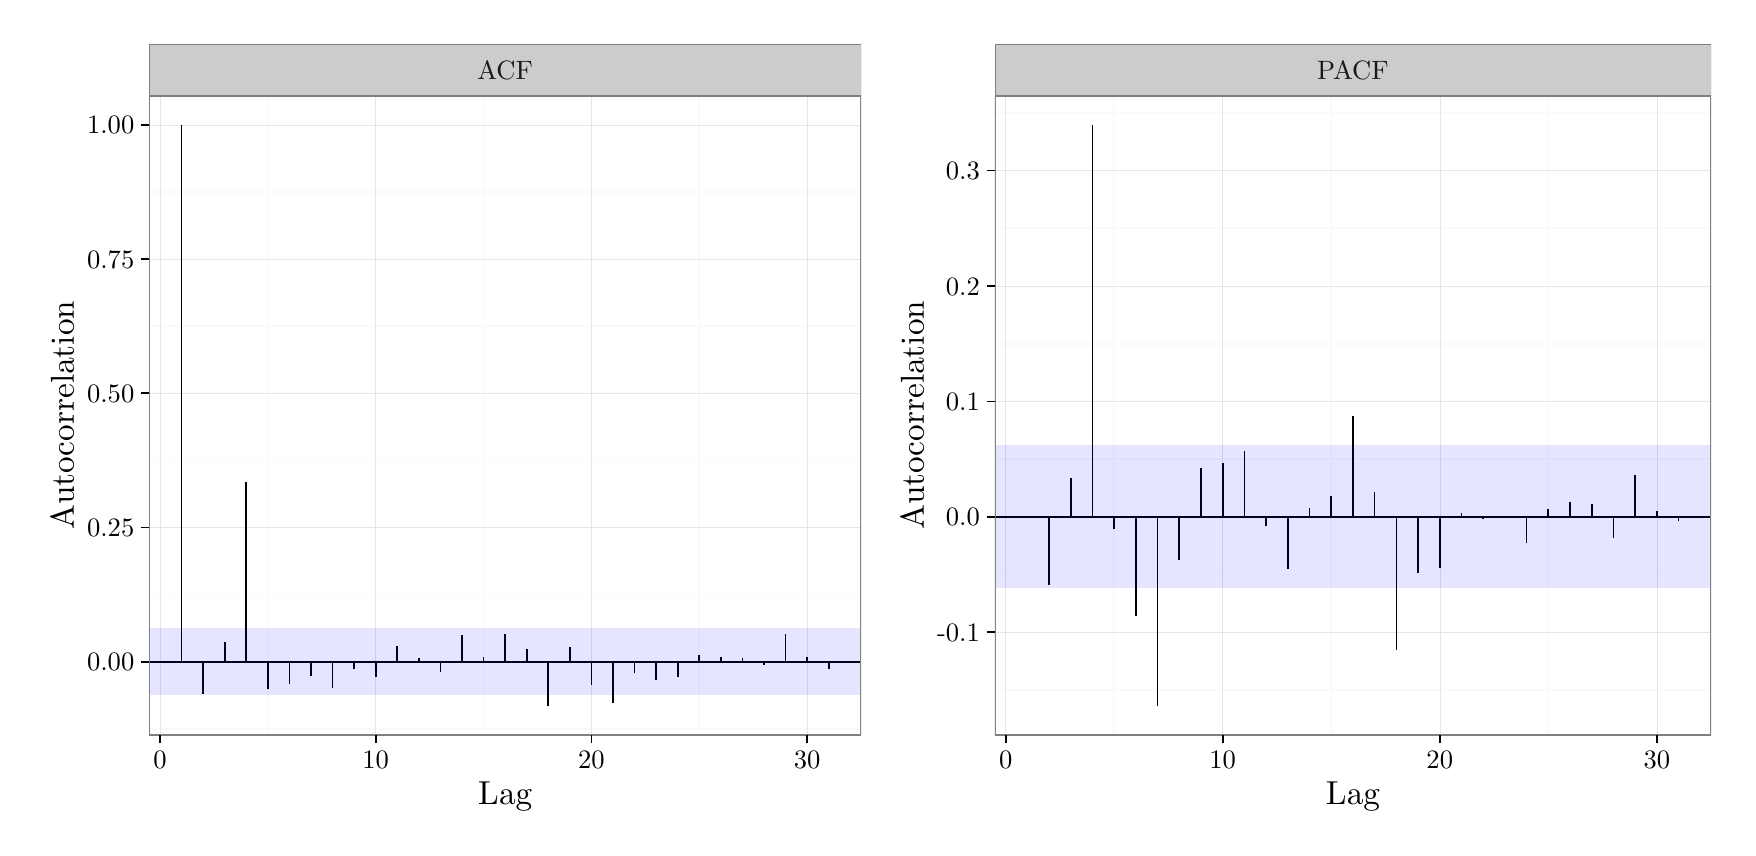
\begin{tikzpicture}[x=1pt,y=1pt]
\definecolor{fillColor}{RGB}{255,255,255}
\path[use as bounding box,fill=fillColor,fill opacity=0.00] (0,0) rectangle (614.29,289.08);
\begin{scope}
\path[clip] (  0.00,  0.00) rectangle (307.15,289.08);
\definecolor{drawColor}{RGB}{255,255,255}
\definecolor{fillColor}{RGB}{255,255,255}

\path[draw=drawColor,line width= 0.6pt,line join=round,line cap=round,fill=fillColor] ( -0.00,  0.00) rectangle (307.15,289.08);
\end{scope}
\begin{scope}
\path[clip] ( 43.93, 33.48) rectangle (301.15,264.47);
\definecolor{fillColor}{RGB}{255,255,255}

\path[fill=fillColor] ( 43.93, 33.48) rectangle (301.15,264.47);
\definecolor{drawColor}{gray}{0.98}

\path[draw=drawColor,line width= 0.6pt,line join=round] ( 43.93, 35.70) --
	(301.15, 35.70);

\path[draw=drawColor,line width= 0.6pt,line join=round] ( 43.93, 84.20) --
	(301.15, 84.20);

\path[draw=drawColor,line width= 0.6pt,line join=round] ( 43.93,132.71) --
	(301.15,132.71);

\path[draw=drawColor,line width= 0.6pt,line join=round] ( 43.93,181.21) --
	(301.15,181.21);

\path[draw=drawColor,line width= 0.6pt,line join=round] ( 43.93,229.72) --
	(301.15,229.72);

\path[draw=drawColor,line width= 0.6pt,line join=round] ( 86.80, 33.48) --
	( 86.80,264.47);

\path[draw=drawColor,line width= 0.6pt,line join=round] (164.74, 33.48) --
	(164.74,264.47);

\path[draw=drawColor,line width= 0.6pt,line join=round] (242.69, 33.48) --
	(242.69,264.47);
\definecolor{drawColor}{gray}{0.90}

\path[draw=drawColor,line width= 0.2pt,line join=round] ( 43.93, 59.95) --
	(301.15, 59.95);

\path[draw=drawColor,line width= 0.2pt,line join=round] ( 43.93,108.45) --
	(301.15,108.45);

\path[draw=drawColor,line width= 0.2pt,line join=round] ( 43.93,156.96) --
	(301.15,156.96);

\path[draw=drawColor,line width= 0.2pt,line join=round] ( 43.93,205.46) --
	(301.15,205.46);

\path[draw=drawColor,line width= 0.2pt,line join=round] ( 43.93,253.97) --
	(301.15,253.97);

\path[draw=drawColor,line width= 0.2pt,line join=round] ( 47.82, 33.48) --
	( 47.82,264.47);

\path[draw=drawColor,line width= 0.2pt,line join=round] (125.77, 33.48) --
	(125.77,264.47);

\path[draw=drawColor,line width= 0.2pt,line join=round] (203.72, 33.48) --
	(203.72,264.47);

\path[draw=drawColor,line width= 0.2pt,line join=round] (281.66, 33.48) --
	(281.66,264.47);
\definecolor{drawColor}{RGB}{0,0,0}

\path[draw=drawColor,line width= 0.6pt,line join=round] ( 43.93, 59.95) -- (301.15, 59.95);

\path[draw=drawColor,line width= 0.6pt,line join=round] ( 55.62,253.97) -- ( 55.62, 59.95);

\path[draw=drawColor,line width= 0.6pt,line join=round] ( 63.41, 48.45) -- ( 63.41, 59.95);

\path[draw=drawColor,line width= 0.6pt,line join=round] ( 71.21, 67.12) -- ( 71.21, 59.95);

\path[draw=drawColor,line width= 0.6pt,line join=round] ( 79.00,124.76) -- ( 79.00, 59.95);

\path[draw=drawColor,line width= 0.6pt,line join=round] ( 86.80, 50.11) -- ( 86.80, 59.95);

\path[draw=drawColor,line width= 0.6pt,line join=round] ( 94.59, 51.98) -- ( 94.59, 59.95);

\path[draw=drawColor,line width= 0.6pt,line join=round] (102.39, 54.97) -- (102.39, 59.95);

\path[draw=drawColor,line width= 0.6pt,line join=round] (110.18, 50.61) -- (110.18, 59.95);

\path[draw=drawColor,line width= 0.6pt,line join=round] (117.98, 57.18) -- (117.98, 59.95);

\path[draw=drawColor,line width= 0.6pt,line join=round] (125.77, 54.28) -- (125.77, 59.95);

\path[draw=drawColor,line width= 0.6pt,line join=round] (133.56, 65.72) -- (133.56, 59.95);

\path[draw=drawColor,line width= 0.6pt,line join=round] (141.36, 61.31) -- (141.36, 59.95);

\path[draw=drawColor,line width= 0.6pt,line join=round] (149.15, 56.31) -- (149.15, 59.95);

\path[draw=drawColor,line width= 0.6pt,line join=round] (156.95, 69.61) -- (156.95, 59.95);

\path[draw=drawColor,line width= 0.6pt,line join=round] (164.74, 61.58) -- (164.74, 59.95);

\path[draw=drawColor,line width= 0.6pt,line join=round] (172.54, 69.91) -- (172.54, 59.95);

\path[draw=drawColor,line width= 0.6pt,line join=round] (180.33, 64.62) -- (180.33, 59.95);

\path[draw=drawColor,line width= 0.6pt,line join=round] (188.13, 43.98) -- (188.13, 59.95);

\path[draw=drawColor,line width= 0.6pt,line join=round] (195.92, 65.45) -- (195.92, 59.95);

\path[draw=drawColor,line width= 0.6pt,line join=round] (203.72, 51.59) -- (203.72, 59.95);

\path[draw=drawColor,line width= 0.6pt,line join=round] (211.51, 44.98) -- (211.51, 59.95);

\path[draw=drawColor,line width= 0.6pt,line join=round] (219.30, 55.78) -- (219.30, 59.95);

\path[draw=drawColor,line width= 0.6pt,line join=round] (227.10, 53.19) -- (227.10, 59.95);

\path[draw=drawColor,line width= 0.6pt,line join=round] (234.89, 54.28) -- (234.89, 59.95);

\path[draw=drawColor,line width= 0.6pt,line join=round] (242.69, 62.47) -- (242.69, 59.95);

\path[draw=drawColor,line width= 0.6pt,line join=round] (250.48, 61.62) -- (250.48, 59.95);

\path[draw=drawColor,line width= 0.6pt,line join=round] (258.28, 61.27) -- (258.28, 59.95);

\path[draw=drawColor,line width= 0.6pt,line join=round] (266.07, 58.85) -- (266.07, 59.95);

\path[draw=drawColor,line width= 0.6pt,line join=round] (273.87, 70.04) -- (273.87, 59.95);

\path[draw=drawColor,line width= 0.6pt,line join=round] (281.66, 61.73) -- (281.66, 59.95);

\path[draw=drawColor,line width= 0.6pt,line join=round] (289.46, 57.38) -- (289.46, 59.95);
\definecolor{fillColor}{RGB}{0,0,255}

\path[fill=fillColor,fill opacity=0.10] ( 43.93, 47.92) rectangle (301.15, 71.97);
\definecolor{drawColor}{gray}{0.50}

\path[draw=drawColor,line width= 0.6pt,line join=round,line cap=round] ( 43.93, 33.48) rectangle (301.15,264.47);
\end{scope}
\begin{scope}
\path[clip] ( 43.93,264.47) rectangle (301.15,283.08);
\definecolor{drawColor}{gray}{0.50}
\definecolor{fillColor}{gray}{0.80}

\path[draw=drawColor,line width= 0.2pt,line join=round,line cap=round,fill=fillColor] ( 43.93,264.47) rectangle (301.15,283.08);
\definecolor{drawColor}{gray}{0.10}

\node[text=drawColor,anchor=base,inner sep=0pt, outer sep=0pt, scale=  0.96] at (172.54,270.47) {ACF};
\end{scope}
\begin{scope}
\path[clip] (  0.00,  0.00) rectangle (614.29,289.08);
\definecolor{drawColor}{RGB}{0,0,0}

\node[text=drawColor,anchor=base east,inner sep=0pt, outer sep=0pt, scale=  0.96] at ( 38.53, 56.64) {0.00};

\node[text=drawColor,anchor=base east,inner sep=0pt, outer sep=0pt, scale=  0.96] at ( 38.53,105.15) {0.25};

\node[text=drawColor,anchor=base east,inner sep=0pt, outer sep=0pt, scale=  0.96] at ( 38.53,153.65) {0.50};

\node[text=drawColor,anchor=base east,inner sep=0pt, outer sep=0pt, scale=  0.96] at ( 38.53,202.16) {0.75};

\node[text=drawColor,anchor=base east,inner sep=0pt, outer sep=0pt, scale=  0.96] at ( 38.53,250.66) {1.00};
\end{scope}
\begin{scope}
\path[clip] (  0.00,  0.00) rectangle (614.29,289.08);
\definecolor{drawColor}{RGB}{0,0,0}

\path[draw=drawColor,line width= 0.6pt,line join=round] ( 40.93, 59.95) --
	( 43.93, 59.95);

\path[draw=drawColor,line width= 0.6pt,line join=round] ( 40.93,108.45) --
	( 43.93,108.45);

\path[draw=drawColor,line width= 0.6pt,line join=round] ( 40.93,156.96) --
	( 43.93,156.96);

\path[draw=drawColor,line width= 0.6pt,line join=round] ( 40.93,205.46) --
	( 43.93,205.46);

\path[draw=drawColor,line width= 0.6pt,line join=round] ( 40.93,253.97) --
	( 43.93,253.97);
\end{scope}
\begin{scope}
\path[clip] (  0.00,  0.00) rectangle (614.29,289.08);
\definecolor{drawColor}{RGB}{0,0,0}

\path[draw=drawColor,line width= 0.6pt,line join=round] ( 47.82, 30.48) --
	( 47.82, 33.48);

\path[draw=drawColor,line width= 0.6pt,line join=round] (125.77, 30.48) --
	(125.77, 33.48);

\path[draw=drawColor,line width= 0.6pt,line join=round] (203.72, 30.48) --
	(203.72, 33.48);

\path[draw=drawColor,line width= 0.6pt,line join=round] (281.66, 30.48) --
	(281.66, 33.48);
\end{scope}
\begin{scope}
\path[clip] (  0.00,  0.00) rectangle (614.29,289.08);
\definecolor{drawColor}{RGB}{0,0,0}

\node[text=drawColor,anchor=base,inner sep=0pt, outer sep=0pt, scale=  0.96] at ( 47.82, 21.46) {0};

\node[text=drawColor,anchor=base,inner sep=0pt, outer sep=0pt, scale=  0.96] at (125.77, 21.46) {10};

\node[text=drawColor,anchor=base,inner sep=0pt, outer sep=0pt, scale=  0.96] at (203.72, 21.46) {20};

\node[text=drawColor,anchor=base,inner sep=0pt, outer sep=0pt, scale=  0.96] at (281.66, 21.46) {30};
\end{scope}
\begin{scope}
\path[clip] (  0.00,  0.00) rectangle (614.29,289.08);
\definecolor{drawColor}{RGB}{0,0,0}

\node[text=drawColor,anchor=base,inner sep=0pt, outer sep=0pt, scale=  1.20] at (172.54,  8.40) {Lag};
\end{scope}
\begin{scope}
\path[clip] (  0.00,  0.00) rectangle (614.29,289.08);
\definecolor{drawColor}{RGB}{0,0,0}

\node[text=drawColor,rotate= 90.00,anchor=base,inner sep=0pt, outer sep=0pt, scale=  1.20] at ( 16.66,148.97) {Autocorrelation};
\end{scope}
\begin{scope}
\path[clip] (307.15,  0.00) rectangle (614.29,289.08);
\definecolor{drawColor}{RGB}{255,255,255}
\definecolor{fillColor}{RGB}{255,255,255}

\path[draw=drawColor,line width= 0.6pt,line join=round,line cap=round,fill=fillColor] (307.15,  0.00) rectangle (614.29,289.08);
\end{scope}
\begin{scope}
\path[clip] (349.48, 33.48) rectangle (608.30,264.47);
\definecolor{fillColor}{RGB}{255,255,255}

\path[fill=fillColor] (349.48, 33.48) rectangle (608.29,264.47);
\definecolor{drawColor}{gray}{0.98}

\path[draw=drawColor,line width= 0.6pt,line join=round] (349.48, 49.84) --
	(608.30, 49.84);

\path[draw=drawColor,line width= 0.6pt,line join=round] (349.48, 91.53) --
	(608.30, 91.53);

\path[draw=drawColor,line width= 0.6pt,line join=round] (349.48,133.21) --
	(608.30,133.21);

\path[draw=drawColor,line width= 0.6pt,line join=round] (349.48,174.89) --
	(608.30,174.89);

\path[draw=drawColor,line width= 0.6pt,line join=round] (349.48,216.57) --
	(608.30,216.57);

\path[draw=drawColor,line width= 0.6pt,line join=round] (349.48,258.26) --
	(608.30,258.26);

\path[draw=drawColor,line width= 0.6pt,line join=round] (392.61, 33.48) --
	(392.61,264.47);

\path[draw=drawColor,line width= 0.6pt,line join=round] (471.04, 33.48) --
	(471.04,264.47);

\path[draw=drawColor,line width= 0.6pt,line join=round] (549.47, 33.48) --
	(549.47,264.47);
\definecolor{drawColor}{gray}{0.90}

\path[draw=drawColor,line width= 0.2pt,line join=round] (349.48, 70.68) --
	(608.30, 70.68);

\path[draw=drawColor,line width= 0.2pt,line join=round] (349.48,112.37) --
	(608.30,112.37);

\path[draw=drawColor,line width= 0.2pt,line join=round] (349.48,154.05) --
	(608.30,154.05);

\path[draw=drawColor,line width= 0.2pt,line join=round] (349.48,195.73) --
	(608.30,195.73);

\path[draw=drawColor,line width= 0.2pt,line join=round] (349.48,237.42) --
	(608.30,237.42);

\path[draw=drawColor,line width= 0.2pt,line join=round] (353.40, 33.48) --
	(353.40,264.47);

\path[draw=drawColor,line width= 0.2pt,line join=round] (431.83, 33.48) --
	(431.83,264.47);

\path[draw=drawColor,line width= 0.2pt,line join=round] (510.26, 33.48) --
	(510.26,264.47);

\path[draw=drawColor,line width= 0.2pt,line join=round] (588.69, 33.48) --
	(588.69,264.47);
\definecolor{drawColor}{RGB}{0,0,0}

\path[draw=drawColor,line width= 0.6pt,line join=round] (349.48,112.37) -- (608.30,112.37);

\path[draw=drawColor,line width= 0.6pt,line join=round] (369.08, 87.66) -- (369.08,112.37);

\path[draw=drawColor,line width= 0.6pt,line join=round] (376.93,126.37) -- (376.93,112.37);

\path[draw=drawColor,line width= 0.6pt,line join=round] (384.77,253.97) -- (384.77,112.37);

\path[draw=drawColor,line width= 0.6pt,line join=round] (392.61,107.84) -- (392.61,112.37);

\path[draw=drawColor,line width= 0.6pt,line join=round] (400.45, 76.65) -- (400.45,112.37);

\path[draw=drawColor,line width= 0.6pt,line join=round] (408.30, 43.98) -- (408.30,112.37);

\path[draw=drawColor,line width= 0.6pt,line join=round] (416.14, 96.77) -- (416.14,112.37);

\path[draw=drawColor,line width= 0.6pt,line join=round] (423.98,129.92) -- (423.98,112.37);

\path[draw=drawColor,line width= 0.6pt,line join=round] (431.83,131.76) -- (431.83,112.37);

\path[draw=drawColor,line width= 0.6pt,line join=round] (439.67,136.10) -- (439.67,112.37);

\path[draw=drawColor,line width= 0.6pt,line join=round] (447.51,109.13) -- (447.51,112.37);

\path[draw=drawColor,line width= 0.6pt,line join=round] (455.36, 93.43) -- (455.36,112.37);

\path[draw=drawColor,line width= 0.6pt,line join=round] (463.20,115.49) -- (463.20,112.37);

\path[draw=drawColor,line width= 0.6pt,line join=round] (471.04,119.68) -- (471.04,112.37);

\path[draw=drawColor,line width= 0.6pt,line join=round] (478.89,148.90) -- (478.89,112.37);

\path[draw=drawColor,line width= 0.6pt,line join=round] (486.73,121.41) -- (486.73,112.37);

\path[draw=drawColor,line width= 0.6pt,line join=round] (494.57, 64.37) -- (494.57,112.37);

\path[draw=drawColor,line width= 0.6pt,line join=round] (502.41, 91.95) -- (502.41,112.37);

\path[draw=drawColor,line width= 0.6pt,line join=round] (510.26, 93.94) -- (510.26,112.37);

\path[draw=drawColor,line width= 0.6pt,line join=round] (518.10,113.80) -- (518.10,112.37);

\path[draw=drawColor,line width= 0.6pt,line join=round] (525.94,111.42) -- (525.94,112.37);

\path[draw=drawColor,line width= 0.6pt,line join=round] (533.79,111.94) -- (533.79,112.37);

\path[draw=drawColor,line width= 0.6pt,line join=round] (541.63,102.78) -- (541.63,112.37);

\path[draw=drawColor,line width= 0.6pt,line join=round] (549.47,115.32) -- (549.47,112.37);

\path[draw=drawColor,line width= 0.6pt,line join=round] (557.32,117.84) -- (557.32,112.37);

\path[draw=drawColor,line width= 0.6pt,line join=round] (565.16,116.84) -- (565.16,112.37);

\path[draw=drawColor,line width= 0.6pt,line join=round] (573.00,104.67) -- (573.00,112.37);

\path[draw=drawColor,line width= 0.6pt,line join=round] (580.84,127.38) -- (580.84,112.37);

\path[draw=drawColor,line width= 0.6pt,line join=round] (588.69,114.32) -- (588.69,112.37);

\path[draw=drawColor,line width= 0.6pt,line join=round] (596.53,110.73) -- (596.53,112.37);
\definecolor{fillColor}{RGB}{0,0,255}

\path[fill=fillColor,fill opacity=0.10] (349.48, 86.53) rectangle (608.29,138.20);
\definecolor{drawColor}{gray}{0.50}

\path[draw=drawColor,line width= 0.6pt,line join=round,line cap=round] (349.48, 33.48) rectangle (608.29,264.47);
\end{scope}
\begin{scope}
\path[clip] (349.48,264.47) rectangle (608.30,283.08);
\definecolor{drawColor}{gray}{0.50}
\definecolor{fillColor}{gray}{0.80}

\path[draw=drawColor,line width= 0.2pt,line join=round,line cap=round,fill=fillColor] (349.48,264.47) rectangle (608.29,283.08);
\definecolor{drawColor}{gray}{0.10}

\node[text=drawColor,anchor=base,inner sep=0pt, outer sep=0pt, scale=  0.96] at (478.89,270.47) {PACF};
\end{scope}
\begin{scope}
\path[clip] (  0.00,  0.00) rectangle (614.29,289.08);
\definecolor{drawColor}{RGB}{0,0,0}

\node[text=drawColor,anchor=base east,inner sep=0pt, outer sep=0pt, scale=  0.96] at (344.08, 67.38) {-0.1};

\node[text=drawColor,anchor=base east,inner sep=0pt, outer sep=0pt, scale=  0.96] at (344.08,109.06) {0.0};

\node[text=drawColor,anchor=base east,inner sep=0pt, outer sep=0pt, scale=  0.96] at (344.08,150.74) {0.1};

\node[text=drawColor,anchor=base east,inner sep=0pt, outer sep=0pt, scale=  0.96] at (344.08,192.43) {0.2};

\node[text=drawColor,anchor=base east,inner sep=0pt, outer sep=0pt, scale=  0.96] at (344.08,234.11) {0.3};
\end{scope}
\begin{scope}
\path[clip] (  0.00,  0.00) rectangle (614.29,289.08);
\definecolor{drawColor}{RGB}{0,0,0}

\path[draw=drawColor,line width= 0.6pt,line join=round] (346.48, 70.68) --
	(349.48, 70.68);

\path[draw=drawColor,line width= 0.6pt,line join=round] (346.48,112.37) --
	(349.48,112.37);

\path[draw=drawColor,line width= 0.6pt,line join=round] (346.48,154.05) --
	(349.48,154.05);

\path[draw=drawColor,line width= 0.6pt,line join=round] (346.48,195.73) --
	(349.48,195.73);

\path[draw=drawColor,line width= 0.6pt,line join=round] (346.48,237.42) --
	(349.48,237.42);
\end{scope}
\begin{scope}
\path[clip] (  0.00,  0.00) rectangle (614.29,289.08);
\definecolor{drawColor}{RGB}{0,0,0}

\path[draw=drawColor,line width= 0.6pt,line join=round] (353.40, 30.48) --
	(353.40, 33.48);

\path[draw=drawColor,line width= 0.6pt,line join=round] (431.83, 30.48) --
	(431.83, 33.48);

\path[draw=drawColor,line width= 0.6pt,line join=round] (510.26, 30.48) --
	(510.26, 33.48);

\path[draw=drawColor,line width= 0.6pt,line join=round] (588.69, 30.48) --
	(588.69, 33.48);
\end{scope}
\begin{scope}
\path[clip] (  0.00,  0.00) rectangle (614.29,289.08);
\definecolor{drawColor}{RGB}{0,0,0}

\node[text=drawColor,anchor=base,inner sep=0pt, outer sep=0pt, scale=  0.96] at (353.40, 21.46) {0};

\node[text=drawColor,anchor=base,inner sep=0pt, outer sep=0pt, scale=  0.96] at (431.83, 21.46) {10};

\node[text=drawColor,anchor=base,inner sep=0pt, outer sep=0pt, scale=  0.96] at (510.26, 21.46) {20};

\node[text=drawColor,anchor=base,inner sep=0pt, outer sep=0pt, scale=  0.96] at (588.69, 21.46) {30};
\end{scope}
\begin{scope}
\path[clip] (  0.00,  0.00) rectangle (614.29,289.08);
\definecolor{drawColor}{RGB}{0,0,0}

\node[text=drawColor,anchor=base,inner sep=0pt, outer sep=0pt, scale=  1.20] at (478.89,  8.40) {Lag};
\end{scope}
\begin{scope}
\path[clip] (  0.00,  0.00) rectangle (614.29,289.08);
\definecolor{drawColor}{RGB}{0,0,0}

\node[text=drawColor,rotate= 90.00,anchor=base,inner sep=0pt, outer sep=0pt, scale=  1.20] at (323.81,148.97) {Autocorrelation};
\end{scope}
\end{tikzpicture}
